%* File            :    MAIN.tex
%*
%* HAUPTDOKUMENT
%*
%* Dieses Dokument bindet alle untergeordneten Dokumente
%* ein. Es wird beim Aufruf von pdflatex als Quelle angegeben.
%*
%* Autoren         :    Daniel Hering, Tobias Wartzek
%*
%* Datum           :    05.12.2009
%***********************************************************************



\documentclass[12pt,a4paper,twoside,openright,index=totoc,listof=totoc,BCOR=8.25mm,headinclude,footinclude=false,headsepline,notitlepage,numbers=noenddot,bibliography=totoc,headings=normal,parskip=full]{scrbook}

%************************************************************************
% Das Package muss leider hier eingebunden werden da sonst in den
% Befehlen f�r hypersetup keinerlei Umlaute zur Verf�gung stehen
%************************************************************************

\usepackage[latin1]{inputenc}            % erlaubt direkte Eingabe Deutscher
                                         % Sonderzeichen in .tex Dateien
                                         %(latin1=iso8859-1 fuer Unix Editoren
                                         % oder Windows Editoren die auch latin1
                                         % beherrschen)

%\usepackage[ngerman, english]{babel}
\usepackage[english]{babel}
\usepackage[T1]{fontenc}
\usepackage{setspace}
\setstretch{1.15}
\usepackage{tabularx}
\usepackage{multirow}
\usepackage{graphicx}
\usepackage{subfig}
\usepackage{booktabs}
%************************************************************************
% Dateiinfos eintragen (u.a. von hypersetup und f�r die Titelseite verwendet)
%************************************************************************
\usepackage{pdfpages}
% Titel der Arbeit
\newcommand*{\doclongtitle}{Modeling and flow control for a left ventricular assist device}

% Art der Arbeit (Diplomarbeit, Studienarbeit, Bachelorarbeit, etc.)
\newcommand*{\docsubject}{Master Thesis}

% Name des Autors
\newcommand*{\docauthor}{Julia Ribbrock}

% E-Mail Adresse des Autors
\newcommand*{\docauthoremail}{julia.ribbrock@rwth-aachen.de}

% Schl�sselworte der Arbeit
\newcommand*{\dockeywords}{MedIT Latex Studienarbeit Diplomarbeit Vorlage}

% Name des Betreuers
\newcommand*{\docsupervisor}{Patrick Borchers, M.Sc.}

\newcommand*{\docauthorfax}{+49 241 80-6-23211}
\newcommand*{\docauthorphone}{+49 241 80-23211}

% Bild auf der Titelseite
\newcommand*{\doctitlepic}{images/Teststand_I.pdf}

% folgende Befehle nicht �ndern!!
\newcommand*{\dochomepage}{www.medit.hia.rwth-aachen.de}
\newcommand*{\docshorttitle}{\doclongtitle}

%**********************************************
%* Pakete (HEADER)                           *
%**********************************************

%************************************************************************
%* File            :    HEADER.tex
%*
%* Einbinden der erforderlichen Package-Dateien.
%* Definition des PDF-Infoblocks (im Acrobat Reader unter
%* Datei/Dokumenteigenschaften/Uebersicht)
%*
%* Autor  	       :    Daniel Hering, Tobias Wartzek
%* Datum           :    07.12.2009
%************************************************************************

\usepackage[T1]{fontenc}
\usepackage{lmodern}
\usepackage{helvet}
%\usepackage{palatino}
%\usepackage{times}


%\usepackage[ngerman]{babel}
\usepackage[english]{babel}     % Deutsche Silbentrennung ...
                                         % Sollte direkt nach documentclass
                                         % geladen werden.
\usepackage{scrpage2}                    % Kopf- und Fusszeilen
\usepackage{ifpdf}                       % PDF Ausgabe oder nicht ?
                                         % Dieses Paket muss ueber dem graphicx
                                         % Paket stehen.

\usepackage{color}                       % farbig drucken
\usepackage{graphicx}                    % alle mgl. Arten von Bildern einbinden
\usepackage{subfigure}
\usepackage{eso-pic}										 % mehrschichtige Seitenlayouts
\usepackage{tikz}												 % Zeichenpaket und Optionen f�r Bilder.

%******************************************************************************************
% Wenn Matlab Plots erstellt werden sollen, muss das folgende package eingebunden werden. *
% Allerdings kann es vorkommen, dass das package noch nicht installiert ist, so dass *
% dies nachinstalliert werden m�sste.

%\usepackage{pgfplots}							 % Einbinden von Matlab-Plots      		*
%\pgfplotsset{compat=newest}
%\usetikzlibrary{plotmarks}
%******************************************************************************************

% Pakete f�r Tabellen
\usepackage{tabularx}                    % Breite Tabellen (seitenbreite)
\usepackage{multicol}                    % \multicols: Mehrspaltig auf einer Seite
\usepackage{hhline}                      % schoenere Doppellinien fuer Tabellen
\usepackage{longtable}                   % Lange Tabellen
\usepackage{multirow}                    % Mehrzeilige Tabellenzellen
\usepackage{colortbl}										 % Farbige Tabellenzeilen

\usepackage[gennarrow]{eurosym}          % Das Eurosymbol - benutzen mit \EUR{1,00} oder \euro{}
\usepackage{amsmath}                     % mathematische Sonderzeichen
\usepackage{amsxtra}
\usepackage{amssymb}                   	 % Zusaetzliche mathematische Symbole
\usepackage{units}											 % Verwendung:
\usepackage{acronym}
\usepackage{scrhack}										 % Beseitigt Inkompatibilit�ten zwischen Komascript und Listings-Paket
\usepackage{listings}										 % Darstellung von Programmcode als Listing
\usepackage{url}
\usepackage[pdfpagelabels]{hyperref}     % Konfiguration ueber hypersetup
                                         % hyperref sollte als eines der
                                         % letzten Pakete eingebunden werden

\usepackage{ragged2e}										 % Links-/rechtsb�ndig und trotzdem passende Zeilenumbr�che





\newcommand{\changefont}[3]{
	\fontfamily{#1} \fontseries{#2} \fontshape{#3} \selectfont}
\changefont{ptm}{m}{n}

%%%%%%%%%%%%%%%%%%%%%%%%%%%%%%%%%%%%%%%%%%%%%%%%%%%%%%%%%%%%%%%%%%%%%%%%%%%%%%%%%%%%%%%
%%%%%%%%%%%%%%%%%%%%%%%%%%%%%%%%%%%%%%%%%%%%%%%%%%%%%%%%%%%%%%%%%%%%%%%%%%%%%%%%%%%%%%%
%**************************************************************************************
%*     																																								*
%* Ab hier folgen Definitionen einiger Einstellungen die nicht 								  			*
%* vom Benutzer ge�ndert werden m�ssen. 																		  				*
%* 																																						  			*
%**************************************************************************************

\definecolor{rwthblue}{rgb}{0,0.4,0.8}    % Das RWTH-Blau
\definecolor{hellgrau}{rgb}{0.9,0.9,0.9} 	% hellgrau

%************************************************************************
%*																																			*
%* F�r die Ausgabe mit pdflatex n�tige Befehle zur sinnvollen Benutzung	*
%* des Hyperref-Pakets. Auch hier sind normal keine Anpassungen durch 	*
%* den Benutzer n�tig 																									*
%*																																			*
%************************************************************************


\ifpdf
  % \Htmlfalse
  \pdfoutput=1

  \hypersetup{
                pdftitle={\docshorttitle, RWTH Aachen},
                pdfauthor={\docauthor},
                pdfsubject={\docsubject},
                pdfkeywords={\dockeywords},
                pdfpagemode={UseNone},
                plainpages={false},
                colorlinks=true,  % die Option colorlinks schaltet um zwischen "Rahmen
                linkcolor=black,	% um link" -> false und "Text farbig" -> true
				        citecolor=black,  % daher sind die Farbdefinitionen n�tig um Links nicht
				        filecolor=black,	% im Text hervorzuheben. (entw. weisse Rahmen oder
        				urlcolor=black		% eben schwarzer Text)
   }
\fi


%*************************************************************
% Die folgenden zwei Zeilen werden ben�tigt sofern Matlab-	 *
% Plots eingebunden werden sollen														 *
%*************************************************************

\newlength\fheight											% ben�tigt zur Einbindung von Matlab-Plots
\newlength\fwidth												% auskommentieren bei nichtbenutzen


%****************************************************************
% Die folgenden zwei Zeilen �ndern die Gr��e der 	        	    *
% Unterschriften um eine klare Abgrenzung zum Text zu erreichen *
%****************************************************************

\setkomafont{caption}{\small}									% Bild-/Tabellenunterschrift �ndern
\setkomafont{captionlabel}{\small\bfseries}


%*******************************************************************
%* Abb. statt Abbildung	/ Tab. statt Tabelle											 *
%*******************************************************************
\addto\captionsngerman{
\renewcommand{\figurename}{Abb.}
\renewcommand{\tablename}{Tab.}
}


%*******************************************************************
%* Vertikaler Abstand vor Chapter �berschrift �ndern  						 *
%*******************************************************************
\renewcommand {\chapterheadstartvskip}{\vspace*{-\topskip}}



%*************************************************************
%*************************************************************
%*																													**
%* 					Beginn des Dokuments 						  							**
%*																													**
%*************************************************************
%*************************************************************

\begin{document}
\begin{sloppypar}                       % sch�ner Blocksatz trotz langer Worte



%*************************************************************
%																														 *
%										 ENDE ALLER DEFINITIONEN 								 *
%																														 *
%*************************************************************


\frontmatter    												%r�mische Nummerierung aktivieren
%***********************************************************************
%* File            :    titel2.tex
%*
%* Titelseite
%*
%* Autor           :    Daniel Hering
%***********************************************************************

\newcommand{\defaultarraystretch}{\arraystretch}

\begin{titlepage}
\enlargethispage{31mm}
%***********************************************************************
%* Definition der Kopfzeile																						 *
%***********************************************************************
\vspace*{-3cm}
\hspace*{-1.8em}
\begin{tabularx}{19cm}{Xl@{}}
\textsf{\textbf{\LARGE{\docsubject}}} & %
\includegraphics[height=45pt]{images/RWTH_Aachen_University}
\\
\mbox{\vspace{-10mm}\colorbox{rwthblue}{\hspace{18.4cm}}
\rule{0pt}{10pt}}
%\vspace{-10mm}\colorbox{rwthblue}{\hspace{12.7cm}}  {
\includegraphics[height=30pt]{images/medit_l_m_blau_meditheadfoot}}
\end{tabularx}

%***********************************************************************
%* Ende der Definition der Kopfzeile																	 *
%***********************************************************************
\vspace*{15mm}
\par
\begingroup
\huge
\leftskip20pt
\noindent \textsf{\LARGE\docauthor\\
\textbf{\huge \docshorttitle}}
\par
\endgroup
\vfill % F�llt die Seite vertikal auf

%***********************************************************************
%* Hier eine zur Diplomarbeit geh�rende Grafik einbinden 							 *
%***********************************************************************
% 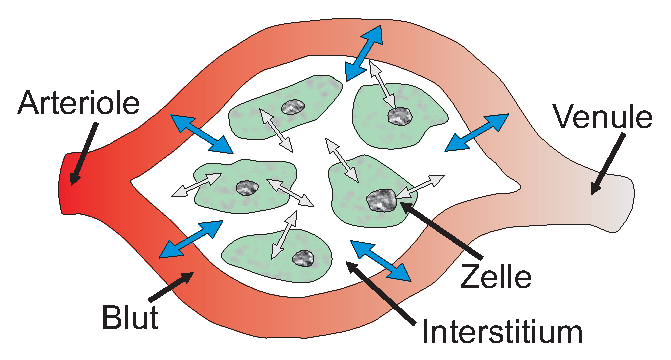
\includegraphics[width=190mm]{images/beispiel1}\vspace{10pt}
%
% \AddToShipoutPicture*{
%      \parbox[b][\paperheight]{\paperwidth}{%
%        \vfill
%         \centering
%         \begin{tikzpicture}[overlay]%
%        		  %\draw[help lines] (0,0) grid (10,20);
%             \node (0,0) [opacity=0.4]{%
%              \hspace{-8,25mm}\includegraphics[width=10cm, height=10cm,keepaspectratio]{\doctitlepic}};%
%          \end{tikzpicture}
%        \vspace{32.35em}
%      }}







\renewcommand{\arraystretch}{1.3}
\hspace*{-1.8em}
\begin{tabularx}{19cm}{Xl}
\multicolumn{2}{l}{\colorbox{rwthblue}{\hspace{18.4cm}}}\\
\multicolumn{2}{l}{\textsf{\textbf{CHAIR FOR MEDICAL INFORMATION TECHNOLOGY}}}\\
\multicolumn{2}{l}{\textsf{{Faculty of Electrical Engineering and Information Technology, RWTH Aachen}}}\\
\multicolumn{2}{l}{\textsf{Univ.-Prof. Dr.-Ing. Dr. med. Dr. h.c. Steffen Leonhardt}}\\
\textsf{Supervisor: \docsupervisor} & \\
\textsf{Date: \today} & \multirow{-2}*~%{
\includegraphics[height=30pt]{images/medit_l_m_blau_meditheadfoot}} \\
\end{tabularx}%}
\renewcommand{\arraystretch}{\defaultarraystretch}

\thispagestyle{empty}
\cleardoublepage

\end{titlepage}

%%***********************************************************************
%* File            :    titel.tex
%*
%* Titelseite 		 
%*
%* Autor           :    Daniel Hering
%***********************************************************************



\let\savedbaselinestretch=\baselinestretch    % Probleme mit geandertem 
                                              % baselinestretch umgehen
\renewcommand{\baselinestretch}{1}%
\begin{titlepage}

%***********************************************************************
%* Definition der Kopfzeile																						 *
%***********************************************************************

\titlehead{\vspace*{-15mm}\underline{\parbox[b]{\textwidth}{
\includegraphics[height=24pt]{images/rwth_logo_blau_rechts}\parbox[b]{0.632\textwidth}{\raggedleft\textcolor{rwthblue}{\footnotesize{HELMHOLTZ-INSTITUT F�R BIOMEDIZINISCHE TECHNIK\\DER RWTH AACHEN}}}
\includegraphics[height=24pt]{images/hia_logo_blau}}}\\\underline{\parbox[b]{\textwidth}{LEHRSTUHL F�R MEDIZINISCHE INFORMATIONSTECHNIK\\Univ.-Prof. Dr.-Ing. Dr. med. Steffen Leonhardt}}}

%***********************************************************************
%* Ende der Definition der Kopfzeile																	 *
%***********************************************************************

\subject{\vspace*{2\baselineskip}}
\title{\docshorttitle}
\author{
  \parbox{.8\linewidth}{%
     \centering\docauthor\\%
\vspace{0.7em}
\large Betreuer/-in: \docsupervisor\\
 \date{\large \today}
}
}%

\publishers{\small\vspace*{\stretch{1000}}%
  \parbox{\linewidth}{%
  \vspace{10cm}
    Pauwelsstra�e 20\\%
    D-52074 Aachen\\%
    Telefon: +49 (0)241 80 -23211\\%
    Fax: +49 (0)241 80 -82442\\%
    E-Mail: medit@hia.rwth-aachen.de\\%
  }%
  \vspace*{-\stretch{1}}%
}
\maketitle
\thispagestyle{empty}
\cleardoublepage
\let\baselinestretch=\savedbaselinestretch%
\end{titlepage}



\cleardoubleemptypage


%**************
%* Danksagung *
%**************

% \chapter{Acknowledgement}
% \thispagestyle{empty}
% As getting to the point of writing this thesis would not have been possible without the great help of some people, i would like to use this as an opportunity to say thanks.
%
% A big thank you goes out to my supervisor, Patrick Borchers (M.Sc.), who has always been at my side with kind words and information, pushing me through the finish line of this thesis.
%
% Furthermore i would like to thank Prof. Dr.-Ing. Dr. Med. Leonhardt, chairman of the chair for medical information technology, for enabling me to write this thesis.
%
% Last but not least, i want to thank all the wonderful people in my daily life, who all stood beside me during these challenging times of my studies, never doubting me especially when i've lost faith in this process.

\cleardoubleemptypage

%************************************************
%* Erkl�rung (hier muss nichts ge�ndert werden) *
%************************************************

%\chapter*{Erkl�rung}
%\thispagestyle{empty}
%\hypertarget{hypsec:erklaerung_der_selbstst}{}%
%
%Ich versichere hiermit, dass ich die vorliegende Arbeit selbstst�ndig
%und ohne Benutzung anderer als der angegebenen Hilfsmittel angefertigt
%habe. Alle Stellen, die w�rtlich oder sinngem�� aus
%ver�ffentlichten und nicht ver�ffentlichten Schriften entnommen
%sind, wurden als solche kenntlich gemacht.\\[3cm]
%
%\begin{tabularx}{\textwidth}{lXl}
%  \rule{5cm}{0.4pt} & & \rule{5cm}{0.4pt}\\
%  Ort, Datum & & Unterschrift
%\end{tabularx}
%\includepdf[angle=90,landscape]{Testbild.png}
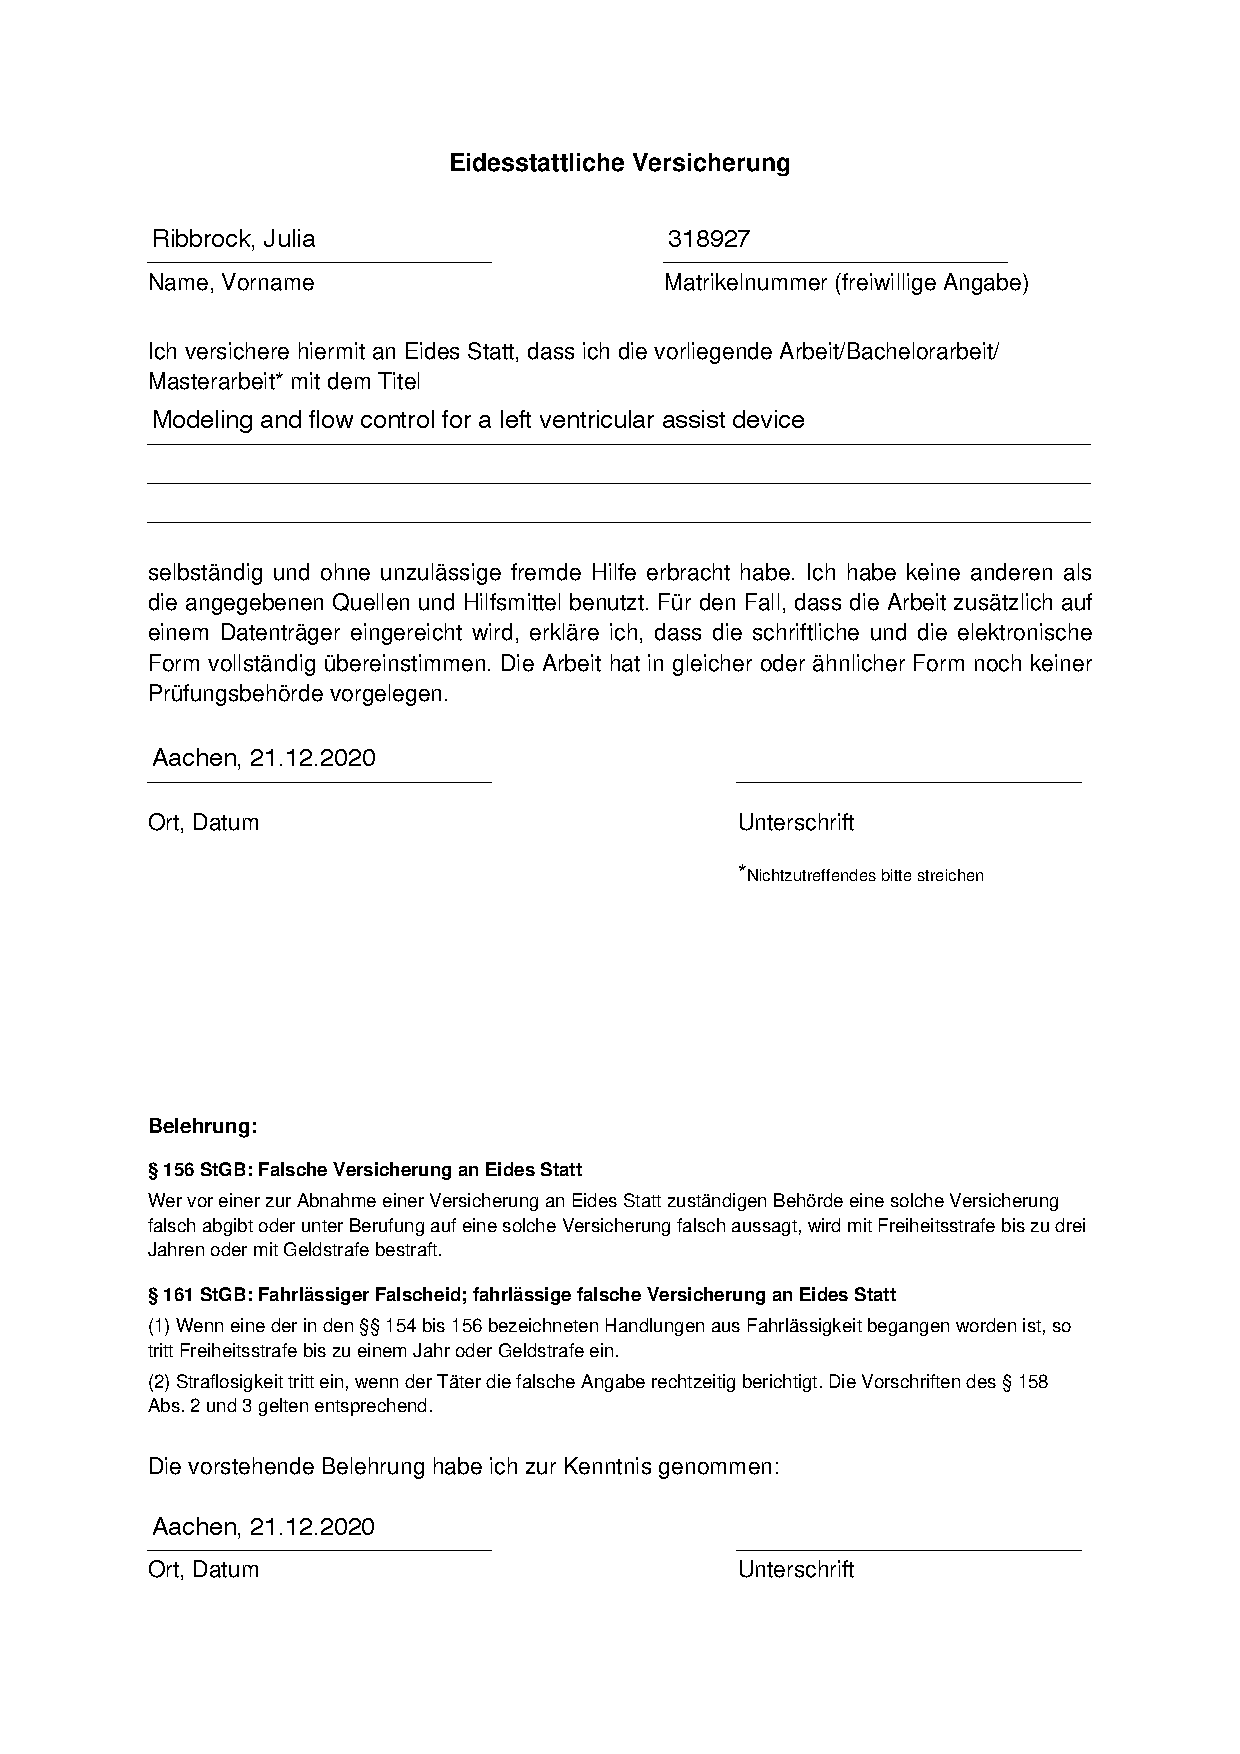
\includepdf{images/Formular_Eidesstattliche_Versicherung_neu}

%\begin{figure}[!ht]
%  \centering
%   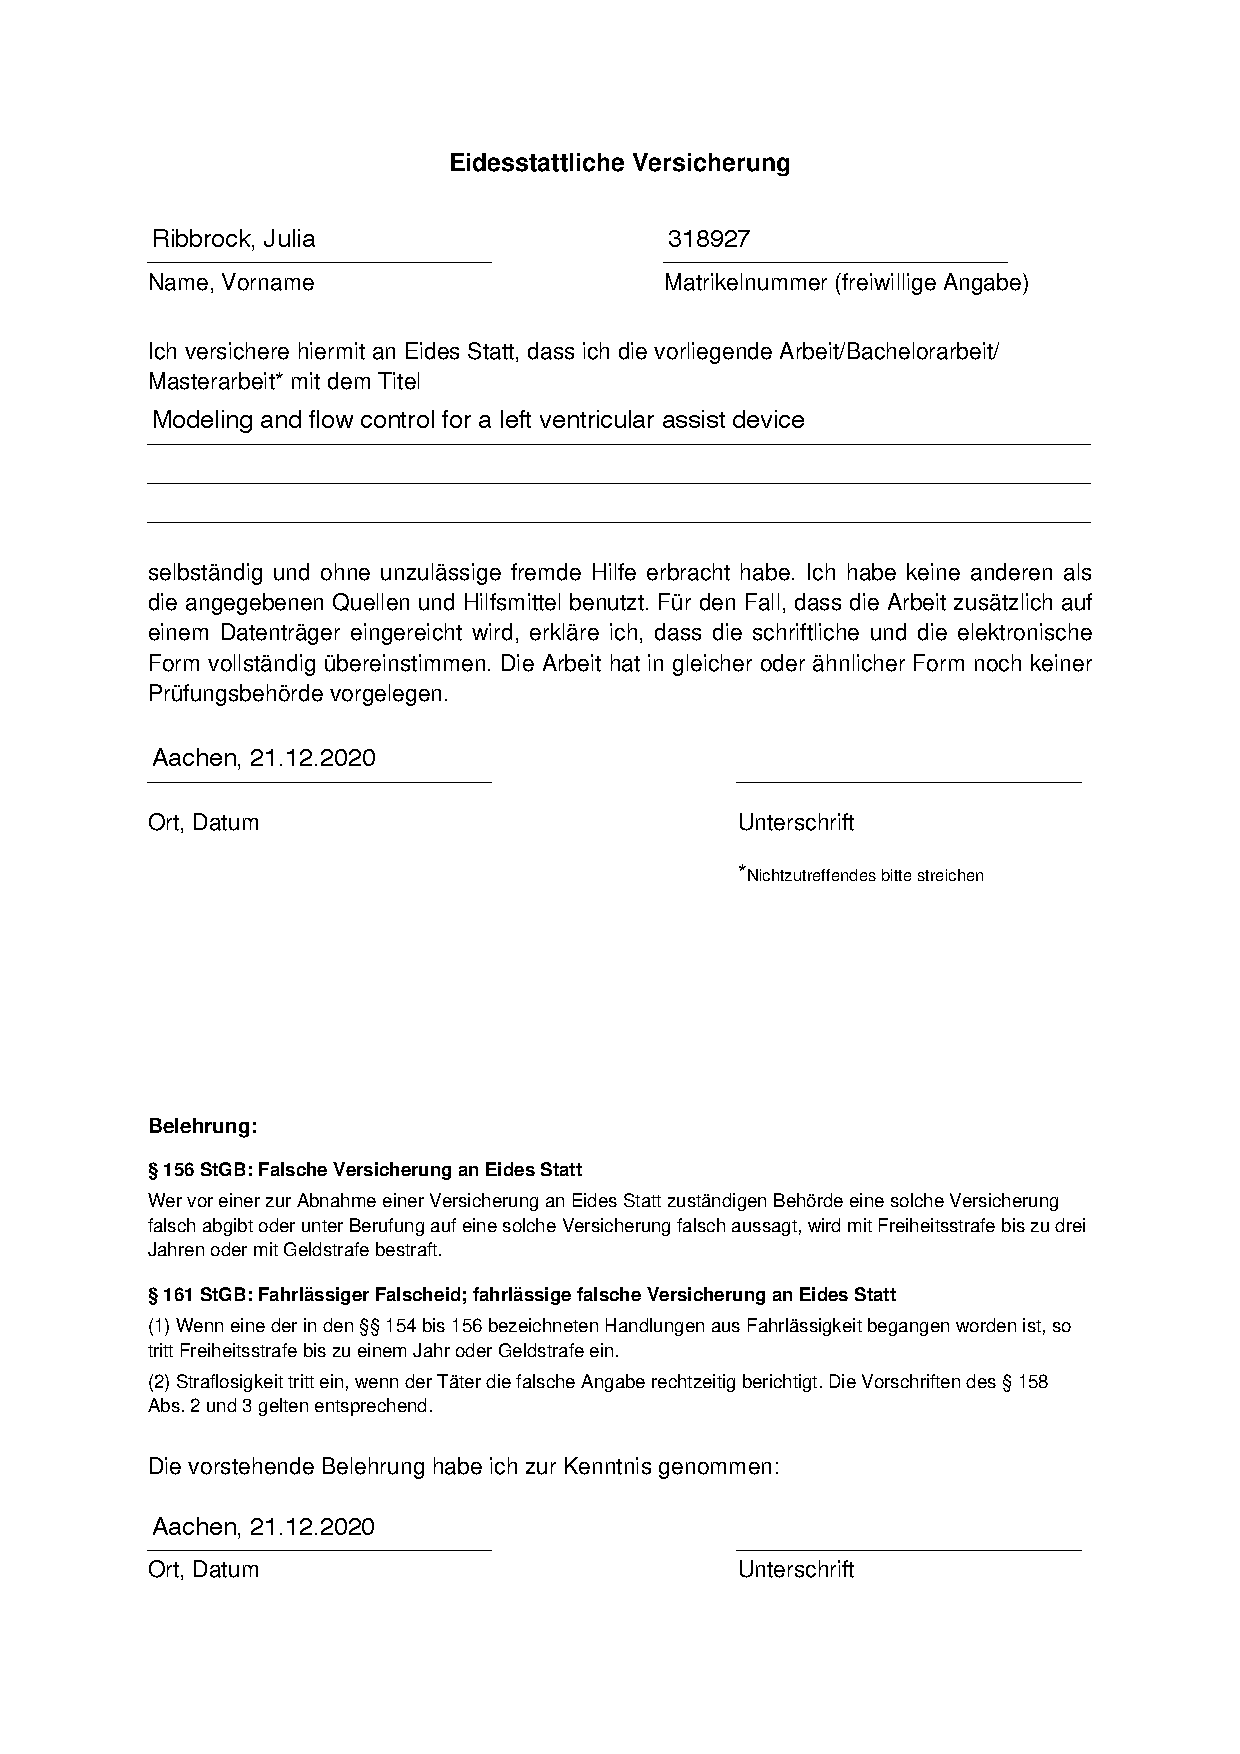
\includegraphics[scale=1]{images/Formular_Eidesstattliche_Versicherung_neu}
%   % Die folgende Anweisungen bindet die Grafik nocheinmal zus�tzlich
%   % als Dateianhang ein. Das hat den Vorteil, dass sie einfach aus dem pdf zur
%   % wieterverwendung extrahierbar ist und der Autor (author) mit angegeben
%   % werden kann. Leider ist die Grafik dadurch auch gleich zweimal im pdf
%   % enthalten und verbraucht dadurch doppelt Platz.
%   % \textattachfile[mimetype=application/pdf,print=false,author=\docauthor,description=\figurename~\ref{fig:beispiel1}]{beispiel1.pdf}{}
%  %% Reihenfolge der Befehle wichtig: zuerst die \caption, danach das \label
%  \label{fig:EidesstattlicheVersicherung}
%\end{figure}

\cleardoubleemptypage

%************
%* Abstract *
%************

\chapter{Abstract}

Acute heart failure is one of the most common reasons for hospitalization due to heart disease. Because end-stage heart failure patients are dependent on a suitable donor heart and the number of cases far exceeds the number of available donor organs, acute heart failure often leads to patient death. Left ventricular assist devices (LVADs) have become a common treatment option for patients with heart failure when drug treatment is no longer sufficient. They assist the patient's heart in its function of pumping blood through the circulatory system and can thus prolong the time for adequate treatment with a donor heart.
\\
The Sputnik VAD is an axial flow pump for left ventricular assistance, recently developed in Russia. Within the scope of this work, a system identification will be performed and different approaches for flow control will be implemented. For the controller implementation, PI controllers are designed according to different methods. Furthermore, the control loop is extended by including various iterative learning controllers. Initially, the goal is to enable regulating the flow to a constant reference. Eventually, however, reference tracking of a variety of reference trajectories is to be enabled. All controller implementations will be tested on a cardiovascular simulator developed at MedIT and their performance will be evaluated afterwards.
\\
For the implementation of the ILCs, the approach of a parallel architecture with a PI controller is chosen.
First, a standard ILC is designed and optimized under optimal, disturbance-free conditions. Based on this ILC, a disturbance in the form of the beating heart, simulated using the cardiovascular system simulator, is included in the control loop. A consideration of the ILC's ability to suppress non-repetitive disturbances revealed potential for improvement. Therefore, an attempt to optimize this capability was implemented in the form of a resampling functionality integrated into the ILC. The evaluation of the measurements showed an increased controller performance.

% VAD6 for abstract/introduction input

\cleardoubleemptypage
\thispagestyle{empty}

\cleardoubleemptypage

%**********************
%* Inhaltsverzeichnis *
%**********************


\addcontentsline{toc}{chapter}{Contents} % Eintrag im Inhaltsverzeichnis erstellen
\tableofcontents                        % Inhaltsverzeichnis anlegen√
\cleardoubleemptypage

%\addcontentsline{toc}{chapter}{List of Figures}
\listoffigures
\cleardoubleemptypage

\listoftables
\cleardoubleemptypage


%*********************
%* Symbolverzeichnis *
%********************

\chapter*{List of Symbols}										% da *-Variante m�ssen Kopfzeilen und TOC-Eintrag von Hand generiert werden
\markboth{List of Symbols}{List of Symbols} 				% Kopfzeile manuell anpassen
\addcontentsline{toc}{chapter}{List of Symbols}				% TOC-Eintrag



\section*{Abbreviations}
%
\acrodef{A-V valve}[A-V valve]{Atrioventricular valve}
\acrodef{BTD}[BTD]{Bridging to decision}
\acrodef{BTR}[BTR]{Bridging to recovery}
\acrodef{BTT}[BTT]{Bridging to transplantation}
\acrodef{BVAD}[BVAD]{Biventricular Assist Device}
\acrodef{CHR}[CHR]{Chien Hrones Reswick}
\acrodef{CO}[CO]{Cardiac Output}
\acrodef{CVDs}[CVDs]{Cardiovascular Diseases}
\acrodef{CVS}[CVS]{Cardiovascular System}
\acrodef{DT}[DT]{Destination therapy}
\acrodef{EDV}[EDV]{End-diastolic volume}
\acrodef{EF}[EF]{Ejection fraction}
\acrodef{ESV}[ESV]{End-systolic volume}
\acrodef{ILC}[ILC]{Iterative learning control}
\acrodef{IMACS}[IMACS]{International Mechanically Assisted Circulatory Support}
\acrodef{INTERMACS}[INTERMACS]{Interagency Registry for Mechanically Assisted Circulatory Support}
\acrodef{HR}[HR]{Heart rate}
\acrodef{HTx}[HTx]{Heart transplantation}
\acrodef{LVAD}[LVAD]{Left Ventricular Assist Device}
\acrodef{MCS}[MCS]{Mechanical Circulatory Support}
\acrodef{RWTH}[RWTH Aachen]{Rheinisch-Westf{\"a}lische Technische Hochschule Aachen}
\acrodef{RVAD}[RVAD]{Right Ventricular Assist Device}
\acrodef{SL valve}[SL valve]{Semilunar valve}
\acrodef{SV}[SV]{Stroke Volume}
\acrodef{VADs}[VADs]{Ventricular Assist Devices}
\acrodef{WHO}[WHO]{World Health Organization}
\acrodef{ZN}[ZN]{Ziegler Nichols}

%* \acs{Name} ruft explizit die Abk�rzung auf.
%* \acl{Name} ruft explizit den ausgeschriebenen Begriff auf.

\begin{tabularx}{\textwidth}{p{.18\textwidth}X}
\acs{A-V valve} & \acl{A-V valve} \\
\acs{BTD} & \acl{BTD} \\
\acs{BTR} & \acl{BTR} \\
\acs{BTT} & \acl{BTT} \\
\acs{BVAD} & \acl{BVAD} \\
\acs{CHR} & \acl{CHR} \\
\acs{CO} & \acl{CO} \\
\acs{CVDs} & \acl{CVDs} \\
\acs{CVS} & \acl{CVS} \\
\acs{DT} & \acl{DT} \\
\acs{EDV} & \acl{EDV} \\
\acs{EF} & \acl{EF} \\
\acs{ESV} & \acl{ESV} \\
\acs{HR} & \acl{HR} \\
\acs{HTx} & \acl{HTx} \\
\acs{ILC} & \acl{ILC} \\
\acs{IMACS} & \acl{IMACS}\\
\acs{INTERMACS} & \acl{INTERMACS}\\
\acs{LVAD} & \acl{LVAD} \\
\acs{MCS} & \acl{MCS} \\
\acs{RWTH} & \acl{RWTH}\\
\acs{SL valve} & \acl{SL valve}\\
\acs{SV} & \acl{SV} \\
\acs{VADs} & \acl{VADs} \\
\acs{WHO} & \acl{WHO} \\
\acs{ZN} & \acl{ZN} \\
\end{tabularx}
%
% \section*{Physikalische Gr��en}
%
% \begin{tabularx}{\textwidth}{p{.18\textwidth}Xp{.1\textwidth}}
% $\mathrm{v}$ & Geschwindigkeit & $\frac{km}{h}$ \\
% $\mathrm{t}$ & Zeit & $h$\\
% \end{tabularx}
%
% \section*{Mathematische Gr��en}
%
% \begin{tabularx}{\textwidth}{p{.18\textwidth}X}
% $\mathrm{M}$ & mathematische Beispielgr��e \\
% \end{tabularx}
%
% \section*{Indizes}
%
% \begin{tabularx}{\textwidth}{p{.18\textwidth}X}
% $k$ & Anzahl der Proze�schritte \\
% $P_{1}...P_{n}$ & Proze�schritt $P_{1}$ bis $P_{n}$\\
% $V_{Ziel}$ &  Zielvektor\\
% \end{tabularx}
%
% \section*{Konstanten}
%
% \begin{tabularx}{\textwidth}{p{.18\textwidth}X}
% $\pi$ & 3.141592653589 \\
% \end{tabularx}

\cleardoubleemptypage

\mainmatter							% Arabische Nummerierung, Beginn des Hauptteils

%**************
%* Einleitung *
%**************

\chapter{Introduction}
\section{Motivation and goal}
\section{Thesis structure}


%*************
%* Hauptteil *
%*************

\chapter{Medical Fundamentals}
Comprehension of the physiology of the human heart and the cardiovascular system is an important prerequisite to the work addressed in this thesis. Therefore, the basics of these topics will be explained in this chapter.

\section{Cardiovascular System}
The fundamental task of the cardiovascular system is to supply all organs with blood. The human cardiovascular system is divided into two components, the systemic circulation and the pulmonary circulation. The systemic circulation is supplying blood flow to all tissues and organs apart from the lungs. \figurename~ \ref{fig:circulation} represents the percentage distribution of the blood over the circulatory system. \cite{GH20}
\begin{figure}[h]
  \centering
  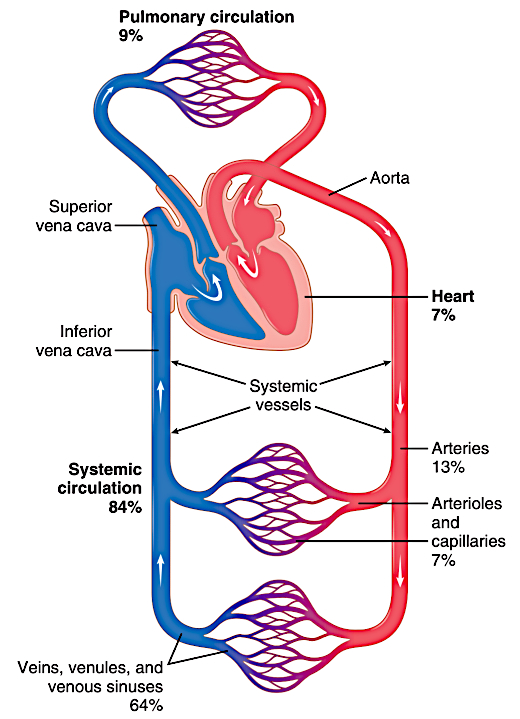
\includegraphics[width=0.5\textwidth, height=0.7\textwidth]{images/circulation.jpg}
  \caption[Blood distribution in the ciculatory system]{Blood distribution in the circulatory system \cite{GH20}.}
  \label{fig:circulation}
\end{figure}
 \\The center of the cardiovascular system is the heart. The heart itself consists of two mechanical pumps, which are functionally connected in series but are united in one organ. It is separated into two sides, which themselves are divided into an atrium and a ventricle each. The atria act as weak primer pumps needed to provide blood flow to the ventricles. \cite{HKS4} Both, the atria and the ventricles are surrounded by the myocardium, which acts as the working muscle of the heart. Through the contraction of the myocardium, blood is pumped into the circulatory system. \cite{HKS7} The left ventricle is pumping oxygenated blood through the aorta into the systemic circulation. There, the oxygen stored in the blood is delivered to the organs. The blood, now low in oxygen, is then led into the right atrium through the inferior and superior vena cava. From the right atrium, the deoxygenated blood then enters the right ventricle. Afterwards it is directed into the pulmonary circulation via the pulmonary artery. After the blood is oxygenated in the lungs, it is returned to the left atrium through the pulmonary vein. \cite{HKS4} In addition to the atria and the ventricles each side of the heart has an atrioventricular (A-V) valve, as well as a semilunar (SL) valve. The A-V valve of the left heart is called the mitral valve, the one of the right heart is referred to as the tricuspid valve. The aortic valve and pulmonary valve are the SL valves of the left and right heart, respectively. The valves determine the direction of blood flow and thus prevent backflow. \cite{HKS7} \figurename~ \ref{fig:heart_anat} provides a graphic overview of the anatomy of the heart and the course of blood flow through the heart.

 \begin{figure}[h]
   \centering
   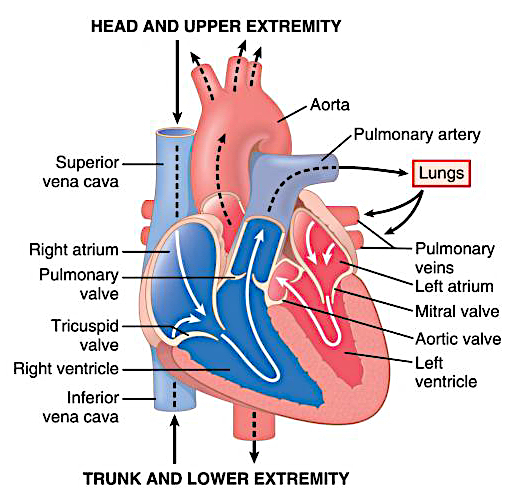
\includegraphics[width=0.7\textwidth]{images/heart_1.jpg}
   \caption[Anatomy of the human heart]{Anatomy of the human heart \cite{GH20}.}
   \label{fig:heart_anat}
 \end{figure}
 %\\
 The amount of blood pumped through the two sides of the heart is equal at all times. This value is called cardiac output (CO). It is determined by multiplying the heart rate (HR) and the stroke volume (SV). For an average adult at rest, with a heart rate of approximately 70 $min^{-1}$ and a stroke volume of 70 $ml$, this leads to
 \begin{equation}
   CO = HR \times SV = 70 min^{-1} \times 70 ml = 5 \frac{l}{min}
  \label{eq:CO}
 \end{equation}
In case of maximum physical load, for a stroke volume of 110 $ml$ and a heart rate of 190 $min^{-1}$,  the cardiac output can increase to up to 20 $\frac{l}{min}$. \cite{HKS4}

The cardiac cycle describes the events that occur during the time-span of one heartbeat. It is triggered by an electrochemical action potential originating from the sinus node. The cycle is divided into four phases. \figurename~ \ref{fig:cardiac_cycle} illustrates these action phases and events of the cardiac cycle for the left ventricle.
\begin{figure}[h]
  \centering
  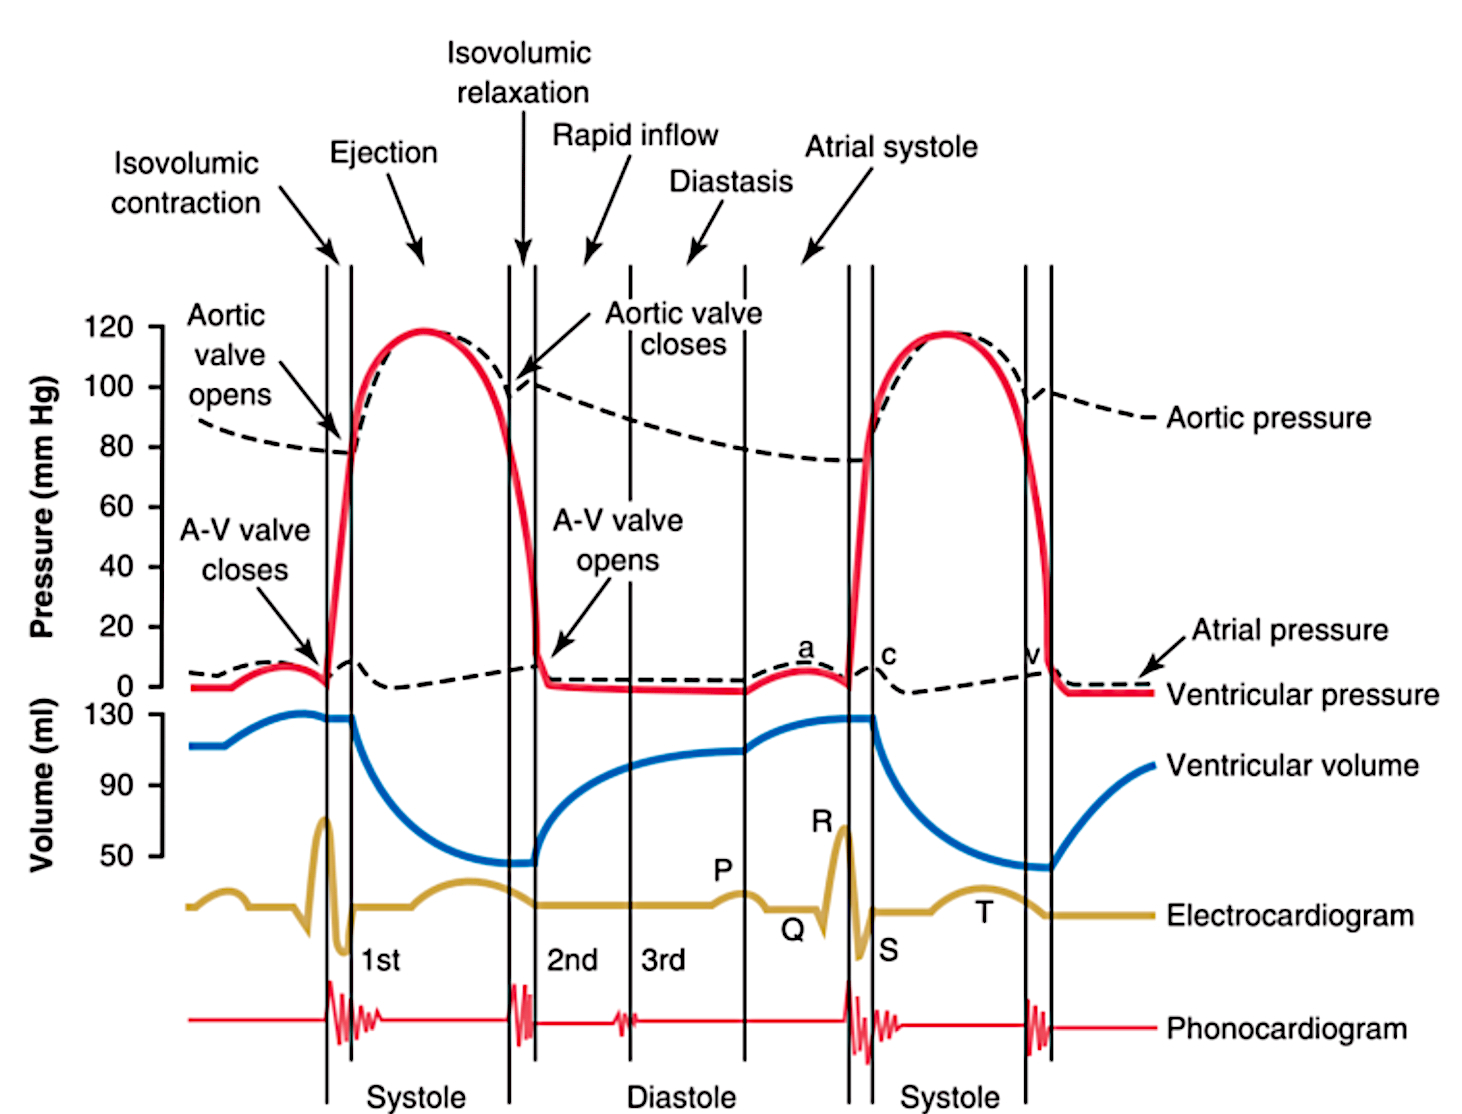
\includegraphics[width=0.8\textwidth]{images/cardiac_cycle.jpg}
  \caption[Action phases of left ventricular cardiac cycle]{Action phases of the cardiac cycle based on the example of the left ventricle \cite{GH20}.}
  \label{fig:cardiac_cycle}
\end{figure}
During the period of isovolumic contraction, the ventricular pressure increases. For the left ventricle, the pressure increases from about 4-6 $mmHg$ to 80 $mmHg$. The pressure values for the right ventricle are much lower. This increase is happening as a direct result of the ventricular contraction. The A-V valves, as well as the SL valves, are closed during this process. This leads to a constant blood volume in the ventricles. As soon as the ventricular pressure exceeds the arterial pressure the pulmonary and aortic valves open and blood can flow into the aorta and the pulmonary artery. This phase is called ejection phase, as the blood is ejected into the circulatory system. The period of isovolumic contraction in combination with the ejection phase describes ventricular systole. \cite{HKS4} During the systole the blood volume in the ventricle decreases by 55-60\%, resulting in an end-systolic volume (ESV) of about 40-50 $ml$ \cite{GH20}. Due to the contraction of the myocardium, the ventricular pressure keeps increasing for a while before decreasing again as the relaxation of the myocardium sets in. As soon as the outflow of the blood ends, the semilunar valves close, initiating the period of isovolumic relaxation. During this period pressure in the ventricles is decreasing, while the blood volume is constant. When the pressure in the atrium exceeds the ventricular pressure, the A-V valves open. This leads to blood flowing into the ventricles until the pressure level in the atria and the ventricles is equalized. \cite{HKS4} This phase is referred to as the period of rapid filling of the ventricles. Combined with the isovolumic relaxation it represents the diastole. The end-diastolic volume (EDV) is about 110-120 $ml$. \cite{GH20} While, at rest, the diastole lasts about twice as long as the systole, above a heart rate of 150 $min^{-1}$, the two phases are about equal \cite{HKS4}.

%\\
The pumping mechanism of the left ventricle can be illustrated well using a pressure-volume diagram (P-V diagram). For the construction of the P-V diagram first the relationship between the left ventricular volume and the ventricular pressure during diastole and systole, as displayed in \figurename~\ref{fig:pv_1}, has to be discussed.
\begin{figure}[h]
  \centering
  \subfloat[]
  {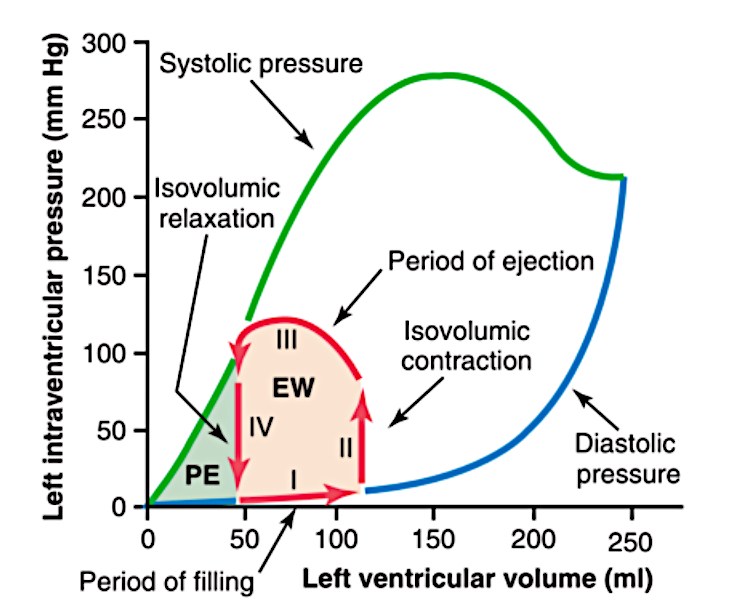
\includegraphics[width=0.5\textwidth]{images/pv_1.jpg}\label{fig:pv_1}}
  \subfloat[]
  {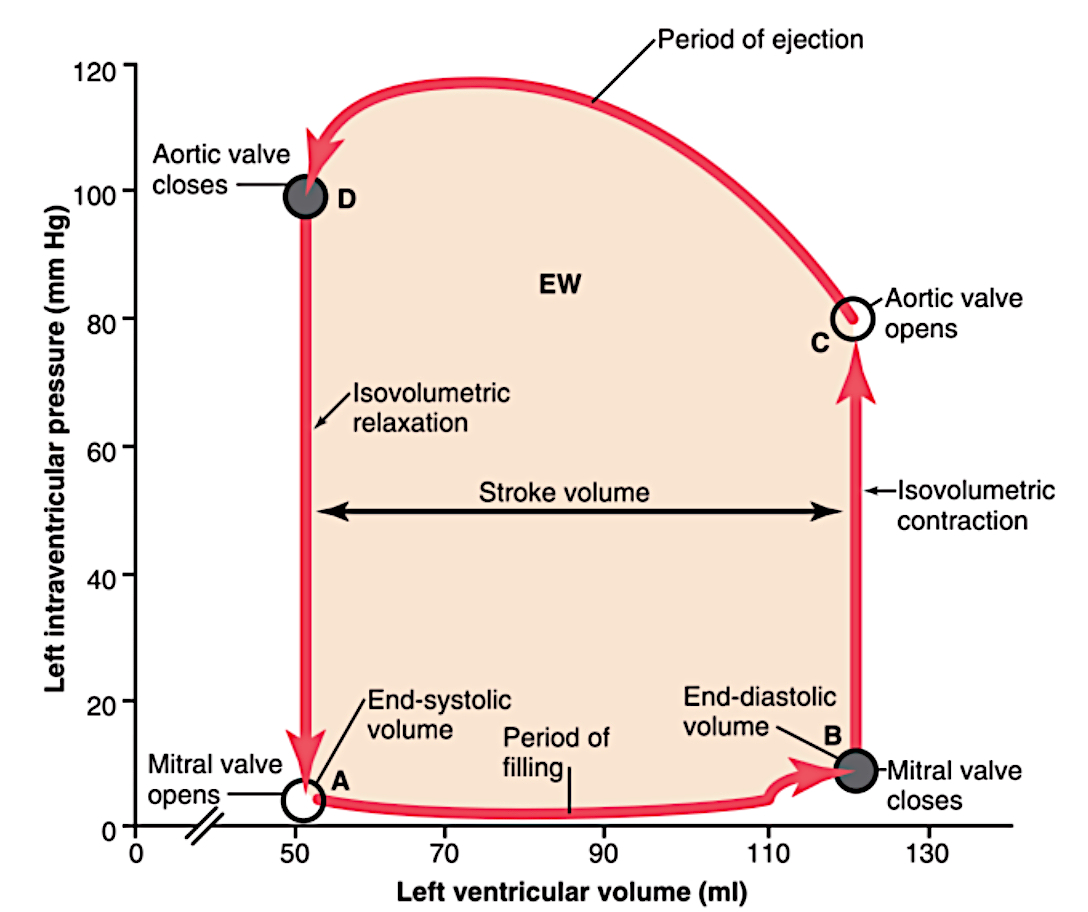
\includegraphics[width=0.5\textwidth]{images/pv_2_.jpg}\label{fig:pv_2}}
  \caption[P-V diagram]{(a)Working diagram of the left ventricle with the P-V diagram. (b) Close-up P-V diagram. \cite{GH20}}
  \label{fig:pv}
\end{figure}
\figurename~\ref{fig:pv_1} displays to curves named \textit{diastolic pressure} and \textit{systolic pressure}. The diastolic pressure is defined as the lowest point of each pulse, in a relaxed state of the heart, while the systolic pressure represents the highest point of each pulse, occuring when the heart is contracting and ejecting blood. \cite{HKS4}
The blue curve, representing the diastolic pressure, is calculated by gradually filling the heart with higher blood volumes and then measuring the diastolic pressure just before ventricular contraction occurs. It is describing the heart's mechanical properties when the myocardium is in a relaxed state. The green curve in \figurename~\ref{fig:pv_1}, named systolic pressure, is plotted by measuring the systolic pressure over varying filling volumes for constant ventricle volumes. The red lines in \figurename~\ref{fig:pv_1} and \figurename~\ref{fig:pv_2} indicate the cardiac cycle and its four action phases, as described above. The line between points A and B in \figurename~\ref{fig:pv_2} depicts the period of rapid filling. The isovolumic contraction is represented through line II in \figurename~\ref{fig:pv_1}, respectively between points B and C in \figurename~ \ref{fig:pv_2}. The ejection phase is represented through III in \figurename~\ref{fig:pv_1} and the line referred to as IV represents the period of isovolumic relaxation. The area of the work diagram, marked with EW in \figurename~\ref{fig:pv} is a measure of the work done by the heart. The P-V diagram furthermore enables calculation of the Ejection Fraction (EF), which describes the percentage value of the ventricle valume ejected during systole. It is determined trough
\begin{equation}
  EF = \frac{SV}{EDV}*100.
 \label{eq:CO}
\end{equation}
For a healthy heart at rest, the EF is at about 50-60 \%.
Knowledge of the P-V diagram is an important prerequisite in understanding myocardial diseases, such as heart failure. For example the EF can decrease to about 20-25 \% in cases of heart failure. \cite{HKS4}

\section{Heart failure}
The World Health Organization (WHO) names cardiovascular diseases (CVDs) as the global number one cause of death. In 2016 about 17.9 million people died from CVDs, which represent 31{\%} of all global death that year. \cite{WHO}
\\In the case of heart failure, the heart is unable to provide the required amount of blood flow to the cardiovascular system in order to supply all organs and tissue with oxygen.
Heart failure does not directly represent a disease but rather a clinical syndrome. Nevertheless, the symptoms of different forms of heart failure are very similar and eventually manifest themselves in a decreased cardiac output. One acute consequence of heart failure, for example, is the feeling of shortness of breath. In the long term, however, severe heart failure can also lead to muscle weakness and a lack of concentration.
\\According to Schmidt et al.\cite{HKS4}, heart failure can be attributed to either systolic dysfunction or diastolic dysfunction. Systolic dysfunction can manifest itself in several ways. One is a reduced contractility and stroke volume of the heart. Causes may be, for example, a coronary artery disease that limits ogxygen supply or a preceding myocardial infarction. Secondly, there may be increased pumping resistance due to an outflow obstruction.  This can be the result of arterial hypertension, among other things. Furthermore, cardiac arrhythmias or a heart attack can lead to systolic dysfunction. \figurename~\ref{fig:sys_dys} displayes the variation of the P-V diagram between a normal functioning heart (dotted line) and one impaired by heart failure with a systolic dysfunction (solid line). In diastolic functional impairment, the dysfunction is evident in the course of the filling phase. This can be triggered, among other things, as a result of reduced compliance of the myocardium due to hypertrophy or fibrosis. The change in the P-V diagram for diastolic heart failure is illustrated in \figurename~\ref{fig:dias_dys}.
\begin{figure}[h]
  \centering
  \subfloat[]
  {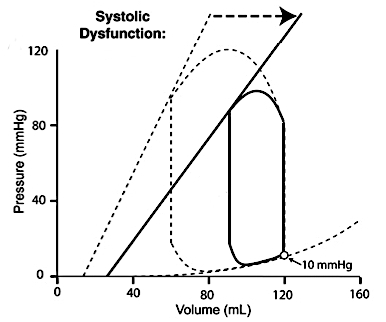
\includegraphics[width=0.5\textwidth]{images/sys_dys.jpg}\label{fig:sys_dys}}
  \subfloat[]
  {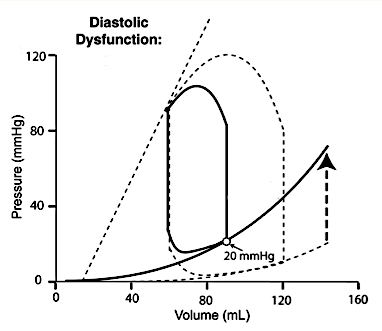
\includegraphics[width=0.5\textwidth]{images/dias_dys.jpg}\label{fig:dias_dys}}
  \caption[P-V diagram for heart failure]{P-V diagram for heart failure in cases of (a) a systolic dysfunction and (b) a diastolic dysfunction according to \cite{HKS_pv}.}
  \label{fig:hf_dys}
\end{figure}

For the treatment of heart failure, drug therapy using beta-blockers is initially targeted in most cases. However, if this is not successful, the use of ventricular assist devices can be a useful alternative in order to relieve the heart and provide sufficient blood flow. \cite{HKS4}

\section{Ventricular Assist Devices}
Despite the fact that heart transplantation (HTx) still is the gold standard for treatment of patients with terminal heart failure \cite{VAD2} ventricular assist devices (VADs), as a kind of mechanical circulatory support (MCS) technology, are becoming more and more important in treating patients with CVDs. There are two reasons for this. On the one hand, CVDs are gaining in importance due to demographic change. On the other hand, there is an increasing shortage of donor organs. \cite{VAD7}

\subsection{Therapeutic objective}
Traditionally the therapeutic goals of VAD treatment can be divided into three categories: \textit{bridging to transplantation} (BTT), \textit{bridging to recovery} (BTR) and \textit{destination therapy} (DT). However in some cases also the classification into \textit{bridging to decision} (BTD) and \textit{bridging to transplantability} are mentioned as well. The decision for one of these goals is based on the type of CVD and the condition the patient is in, when receiving VAD assistance. \cite{VAD6} In clinical praxis different classification techniques connecting the patient condition, with the estimated survial time and the need for VAD assistance are used. An overview on the relation between the INTERMACS Score, the New York Heart Association(NYHA)-classification and the patient's condition is presented in \tablename~ \ref{tab:Table1}.
\begin{table}
  \begin{tabularx}{\textwidth}{l|c|l|l}
    \toprule
    INTERMACS & NYHA & Patient condition & Survival time  \\
    Score & & &\\
    \midrule
    1 & IV & critical cardiogenic shock & hours \\
    2 & IV & increasing catecholamine demand & days \\
    3 & IV & stable under inotropics & a week \\
    4 & IV & frequent decompensation & weeks-month \\
    5 & IV & rest discomfort/ not resilient & weeks-month \\
    6 & IV & rest discomfort/ merely resilient & month \\
    7 & IIIb & merely resilient & one year survival rate: \\
     & & & 50-70\% \\
     \bottomrule
  \end{tabularx}
  \caption[Relation between INTERMACS Score and NYHA-classification]{Relation between INTERMACS Score, NYHA-classification, patient condition and approximate survival time based on \cite{VAD5}.}
  \label{tab:Table1}
\end{table}
The INTERMACS Score, which is based on data from patients which have received VAD treatment, links the need for a VAD and the appropriate time frame in which the devices needs to be implanted. It is of high importance in the decision of the therapeutic objective for VAD treatment. \cite{VAD7}
\\The goal of \textit{bridging to transplantation} has a big relevance with patients in NYHA-IV Stadium which are showing hemodynamical instability. Due to a heart transplantation being the desired final treatment for these patients there must be no contraindication to HTx. In case the patient does show a contraindication, such as malignant tumors or an uncontrollable sepsis, the therapeutic objective changes from BTT to DT. In order for a treatment with a VAD as destination therapy being indicated all conservative treatment options need to be exhausted. Due to the ever-growing shortage of donor organs DT as a therapeutic approach in patients with heart insufficiency will become more relevant in the future even in cases usually suited for heart transplantation. \cite{VAD7} There may occur some cases, in which at first a contraindication for HTx exists, which later on may dissolve. These indicate a therapy based on a \textit{bridging to transplantability} goal. \cite{VAD6}
\\The indication for a \textit{bridging to recovery} approach is twofold. Either the patient shows heart failure as a result of ischemia reperfusion damage or due to infectious genesis. In the first case the myocardium usually is able to recover within a few days, whereas in the second one the potential and the time necessary for recovery depends on how badly the tissue is damaged. In either scenario a weaning from the VAD is an essential part of therapy. \cite{VAD7}
\\If a patient is admitted in cardiogenic shock and medical treatment is not sufficient, \textit{bridging to decision} becomes a relevant form of therapy. By providing the patient with a VAD, a more accurate assessment of the patient's condition is possible.
Based on this, the decision on further treatment can be thought through more thoroughly. \cite{VAD6}

\subsection{Technology}
Since the first artificial blood-pump has been implanted in 1963 \cite{VAD9} technology of VADs has improved significantly.
\\The general aim of ventricular assist devices is to provide mechanical support in pumping blood through the human body with the heart remaining inside the patients body. Despite there being several types of VADs, all of them are working according to the same principle. Blood is taken from the circulatory system through the pumps inlet and ejected at another location via the outlet of the pump.\cite{VAD1}
\\VADs are differentiated by three criteria: the localization of the device inside the human body, the flow profile and the implantation strategy.
\\Regarding the localization of the assistance device there are three types of VADs. With around 93{\%} of all implemented devices the most commonly used ones are the left ventricular assist devices (LVADs). \cite{VAD7} LVADs are placed inside the left ventricle, from where they are pumping blood into the aorta \cite{VAD4}. The second localization option is given by placing the device as a support for  the right ventricle. These devices are therefore called right ventricular assist devices (RVADs). RVADs are positioned in a way that blood is taken from the right atrium and ejected into the pulmonary artery. \cite{VAD7} In some cases RVADs in combination with the aforementioned LVADs are used to build a biventricular assist device (BVAD). This type of heart support is mainly used for more severe heart diseases with a high risk of developing right heart failure. \cite{VAD11}
\\The flow profile as the second criterion for VAD distinction is represented through pulsatile and continuous flow devices. Assistance with pulsatile devices can either be implemented to support the heart in a counter pulsation approach, working synchronous to the heart cycle, or as an asynchronous support. The most commonly known type of pulsatile device is a pneumatically driven pump ventricle. \cite{VAD1}
However, according to the Interagency Registry for Mechanically Assisted Circulatory Support (INTERMACS) over 95{\%} of all implanted devices are continuous flow devices \cite{VAD8}. These, in their most commonly used form, are electrically driven rotational blood pumps. A technological difficulty with these devices is the high probability of blood damage due to small gaps and very high rotational speed. In exchange for this problematic these devices enable a dynamic adaption to the patients physiological needs by being able to quickly adjusting parameters like the motor current. The possibility of keeping track of these signal characteristics furthermore makes it possible to detect malfunctions such like misplacement of the pump. \cite{VAD1}
\\Implantation of the VADs can be performed in one of three ways: paracorporeal, intracorporeal or percutaneous \cite{VAD7}. For VAD systems which follow a paracorporeal approach, only the in- and outflow cannulas are located inside the human body. The cannulas are connecting the pump, which is located outside the body, with the ventricle and the vessels. Due to the pump being placed outside of the patients body, these systems provide the option for pediatric MCS. For most other systems this is not possible due to the device being to big to fit inside a child's body. \cite{VAD10} One example for paracorporeal systems are the aforementioned pneumatically driven pump ventricles \cite{VAD1}. As far as the other two criteria for VAD differentiation are concerned, all combinations of localization and flow control are possible \cite{VAD10}. As an example of a percutaneous device, \cite{VAD7} names the Impella 2.5, which is a rotary blood pump with continuous flow used for left ventricular assistance. \tablename~ \ref{tab:Table2} illustrates the proportions of different VAD types and therapeutic goals using the International Mechanically Assisted Circulatory Support (IMACS) register.
\begin{table}
  \centering
  \begin{tabular}{cc|cc}
    \toprule
    \multicolumn{2}{c|}{VAD type} &
    \multicolumn{2}{c}{Therapeutic objective} \\
    \midrule
    LVAD & 93\% & DT & 40\%\\
    BVAD & 4\% & BTD & 30\%\\
    TAH & 2\% & BTT & 29\%\\
    unknown & 0.1\% & others (BTR, ...) & 1\%\\
    RVAD & 0.05\% & &\\
    \bottomrule
\end{tabular}
  \caption[Distribution of VAD types and therapeutic objectives]{Percentages of VAD types and therapeutic objectives in mechanical heart support based on \cite{VAD7}.}
  \label{tab:Table2}
\end{table}

% \chapter{Technical Fundamentals}
% Since the main part of this thesis addresses the implementation of flow control algorithms for a left ventricular assist device, the basics of control theory and a introduction on iterative learning control will be presented here as well.

\chapter{Control Theory}
Since the field of control theory is a very extensive one, this section will only deal with the fundamentals of notation and structure of a standard control loop. Furthermore, the basic principles of PI-controllers and  iterative learning control (ILC) are discussed, since these are used within the pratical part of the thesis.
\section{Fundamentals}
The basic task of control engineering is to influence a time-varying process from the outside with the goal that the process is executed in a predetermined manner. A control system is characterized in particular by the feedback of the controlled variable to the reference variable. The reference variable represents the state to be achieved.
In theory, this is represented by a control loop with the components shown in \figurename~{\ref{fig:control_loop}}.
\begin{figure}
  \centering
  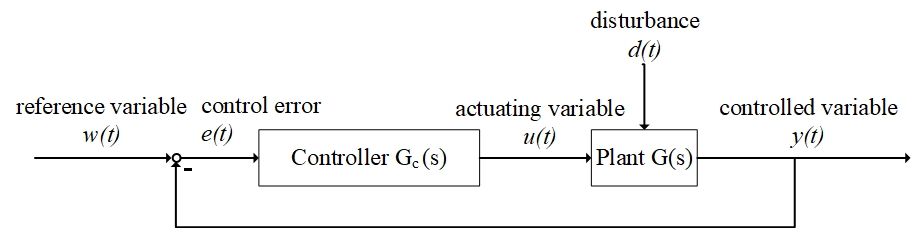
\includegraphics[width=0.9\textwidth]{images/control_loop.jpg}
  \caption[General structure of a control loop]{General structure of a control loop}
  \label{fig:control_loop}
\end{figure}
The plant $G(s)$ transfers the actuating variable $u(t)$, as well as the influence of the the disturbance $d(t)$, to the controlled variable $y(t)$. This variable is permanently compared with the reference variable $w(t)$ by means of a feedback. This feedback provides the control error
\begin{equation}
  e(t) = w(t) - y(t).
 \label{eq:e_t}
\end{equation}
The controller $G_{c}(s)$ then transfers the control error to the actuating variable again. The aim of the control loop is to achieve the smallest possible control error with the highest possible damping. Since these goals contradict each other, a trade off must always be accepted here.\cite{Reg_17}
\\However, there are some general requirements for the closed control loop, which have to be fulfilled. The first of which states that the closed loop needs to be stable. This requirement is met if the control loop responds to a finite excitation with a finite output signal. The second condition is the requirement for disturbance rejection, stating that the controlled variable needs to follow the reference variable asymptotically, so that
\begin{equation}
    \lim\limits_{t \rightarrow \infty}{e(t)} = 0.
 \label{eq:lim_e}
\end{equation}
Another requirement is that the dynamic relationship between the reference variable $w(t)$ and the controlled variable $y(t)$ must satisfy specified quality requirements.  The last requirement states that the first three requirements must be satisfied despite uncertainties in the plant. This requirement is called the robustness requirement. More detailed information on these requirements can be found in \cite{Reg_10}.

The plant $G(s)$ corresponds to the part of the system in which the physical quantity to be controlled is influenced by the controller. The calculation of the plant, by setting up and solving differential equations, is possible only in a few cases. Due to this, the determination of the plant's characteristic values is usually carried out experimentally. There are several basic types of plants. These are classified according to their dynamic behavior. As only the PT$_{1}$-element is used in the practical part of this thesis, all other variations will not be discussed at this point. Detailed information on this topic can, once more, be found in \cite{Reg_10}.
\\The PT$_{1}$-element is the plant type which is most common in technical equipment. A PT$_{n}$-element, in it's static state, reacts proportionally to the input value and has a distinct transition behavior. The index n describes the system order. A PT$_{1}$-element therefore is a proportional delay element of first order. The mathematical formulation of the transfer function of a PT$_{1}$-element is
\begin{equation}
    G(s) = \frac{k_{s}}{1+sT}.
 \label{eq:tf_pt1}
\end{equation}

\begin{figure}[h]
   \centering
   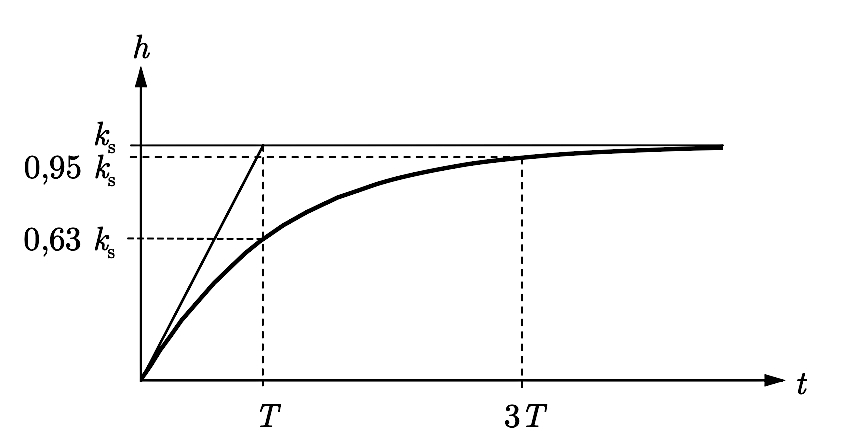
\includegraphics[width=0.9\textwidth]{images/tf_pt1.jpg}
   \caption[Tranfer function of a PT$_{1}$-element]{Transfer function of a PT$_{1}$-element \cite{Reg_10}.}
   \label{fig:tf_pt1}
 \end{figure}
The value $k_{s}$ describes the static gain, which equals the final value of the transfer function. The time constant T enables an impression of the speed with which the system can react to changes at the input. It is defined as the time at which the transfer function reaches 63\% of it's static gain. \cite{Reg_10}
\figurename~\ref{fig:tf_pt1} shows the tranfer function of a PT$_{1}$-element and it's significant parameters.


\section{PI-controller}
A PI-controller is a control structure commonly used for linear systems. This structure consists of both a propotional and an integral control element.
The output value of a P-controller is proportional to it's input value. In relation to the control loop in \figurename~\ref{fig:control_loop} this leads to
\begin{equation}
    u(t) = K_{P}e(t).
 \label{eq:p_contr_1}
\end{equation}
Using Laplacetransformation the transfer function for a P-controller can be determined as
\begin{equation}
    G(s) = \frac{u(s)}{e(s)} = K_{P}
 \label{eq:p_contr_2}
\end{equation}
Therefore, the step response of this controller equals a step weighted with the Parameter $K_{P}$.
The relationship between input and output value of an I-controller is described through
\begin{equation}
    u(t) = K_{I}\int e(t) dt.
 \label{eq:i_contr_1}
\end{equation}
Just as with the P-controller, Laplacetransformation can be used to determine the transfer function of the I-controller.
This leads to
\begin{equation}
    G(s) = \frac{u(s)}{e(s)} = \frac{K_{I}}{s},
 \label{eq:i_contr_2}
\end{equation}
which indicates a step response in form of a ramp with slope $K_{I}$.
In order to generate a PI-controller these elements can be added, which leads to
\begin{equation}
    u(t) = K_{P}e(t) + K_{I}\int e(t) dt.
 \label{eq:pi_contr_1}
\end{equation}
The Laplacetransformation can be used again to formulate the transfer function
\begin{equation}
    G(s) = \frac{u(s)}{e(s)} =  K_{P} + \frac{K_{I}}{s}.
 \label{eq:pi_contr_2}
\end{equation}
The step response of the PI-controller, illustrated in \figurename~\ref{fig:step_resp_pi}, shows both the weigthed step from the P-controller and the ramp from the I-controller.

\begin{figure}[h]
   \centering
   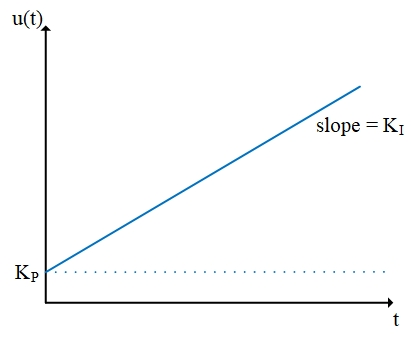
\includegraphics[width=0.4\textwidth]{images/step_resp_pi.jpg}
   \caption[Step response of a PI-Controller]{Step response of a PI-Controller}
   \label{fig:step_resp_pi}
 \end{figure}

\subsection{Tuning rules}
In regards to the controller parameters, tuning is of great importance. If the parameters are chosen incorrectly it can lead to unstable system behavior, which may result in system damage. There are many different approaches to tuning a PI-Controller in order to achieve the best system performance. These are reaching from heuristic methods, over analysis of pole-zero plots, to computer-aided numerical parameter optimization. \cite{Reg_10} At this point only the tuning rules according to Ziegler Nichols (ZN) and the rules according to Chien Hrones Reswick (CHR) will be discussed, as these have been used for the implementation of flow control in the practical work.  Information on other approaches can be found in \cite{Reg_11}.

\subsubsection{Tuning rules according to Ziegler Nichols}
The tuning rules according to Ziegler Nichols are one of the most commoly used heuristic methods in tuning controller parameters for PID-controllers. They are used especially, if a mathematical model of the plant is not available, but the plant can be approximated as a PT$_{n}$-element. \cite{Reg_17}
A necessary condition for this is that the step response of the plant needs to be experimentally identifiable without risk of damage to the system. After the step response has been determined it is displayed graphically. Then the inflection tangent is drawn into the step response as shown in \figurename~\ref{fig:param_zn}.
\begin{figure}
   \centering
   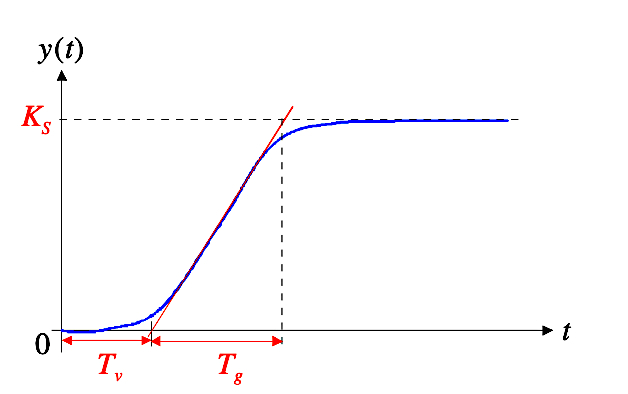
\includegraphics[width=0.7\textwidth]{images/param_zn.jpg}
   \caption[Inflection tangent method Ziegler Nichols]{Inflection tangent method Ziegler Nichols}
   \label{fig:param_zn}
 \end{figure}
The gain $K_{P}$, the delay time $T_{v}$ and the settling time $T_{g}$ can be read from the graph.
The calculation of the controller parameters is performed according to the data in \tablename~\ref{tab:param_zn}. The factor $K_{p}$ from the table equals the term $K_{p}$ in (\ref{eq:pi_contr_2}), while the factor $K_{I}$ is calculated according to:
\begin{equation}
    K_{I}  = \frac{K_{P}}{T_{N}}.
 \label{eq:K_I}
\end{equation}
\begin{table}
  \centering
  \begin{tabularx}{0.6\textwidth}{c|c|c|c}
    \toprule
    Controller type & $K_{P}$ &  $T_{N}$ & $T_{D}$   \\
    \midrule
    P-Controller &  $\frac{T_{g}}{K_{S}T_{v}}$ & - & - \\
    & & & \\
    PI-Controller & $0.9\frac{T_{g}}{K_{S}T_{v}}$ & $3.33T_{v}$ & - \\
    & & & \\
    PID-Controller & $0.9\frac{T_{g}}{K_{S}T_{v}}$ & $2T_{v}$ & $0.5T_{v}$ \\
     \bottomrule
  \end{tabularx}
  \caption[Tuning parameters Ziegler Nichols]{Tuning parameters according to Ziegler Nichols}
  \label{tab:param_zn}
\end{table}

\subsubsection{Tuning rules according to Chien Hrones Reswick}
The tuning method according to Chien Hrones Reswick is a very similar one to the one by Ziegler Nichols. However, this method provides the ability to adjust the transient response of the control loop. The tuning parameters can either be chosen in a way to provide an over damped behavior or a course providing 20\% overshoot. \cite{Reg_11}
For both options the step response and its inflection tangent is graphically displayed, as for the Ziegler Nichols approach in \figurename~\ref{fig:param_zn}.
The values for $K_{P}$, $T_{v}$ and $T_{g}$ are read from the plot. The parameter value $K_{I}$ again is calculated following (\ref{eq:K_I}). \tablename~\ref{tab:param_chr} gives the formulas for calculation of $K_{P}$,  $T_{N}$ and $T_{D}$.

\begin{table}
  \centering
  \begin{tabular}{c|ccc|ccc}
    \toprule
     & \multicolumn{3}{c|}{over damped} & \multicolumn{3}{c}{20\% overshoot} \\
    \midrule
    Controller type & $K_{P}$ &  $T_{N}$ & $T_{D}$ & $K_{P}$ &  $T_{N}$ & $T_{D}$ \\
    \midrule
    P-Controller & $0.3\frac{T_{g}}{K_{S}T_{v}}$ & - & - & $0.7\frac{T_{g}}{K_{S}T_{v}}$ & - & - \\
    & & & & & & \\
    PI-Controller & $0.35\frac{T_{g}}{K_{S}T_{v}}$ & $1.2T_{v}$ & - & $0.6\frac{T_{g}}{K_{S}T_{v}}$ & $T_{v}$ & - \\
        & & & & & & \\
    PID-Controller & $0.6\frac{T_{g}}{K_{S}T_{v}}$ & $T_{v}$ & $0.5T_{v}$ & $0.95\frac{T_{g}}{K_{S}T_{v}}$ & $1.35T_{v}$ & $0.47T_{v}$\\
    \bottomrule
\end{tabular}
  \caption[Tuning parameters Chien Hrones Reswick]{Tuning parameters according to Chien Hrones Reswick}
  \label{tab:param_chr}
\end{table}

\section{Iterative Learning Control}
The use of iterative learning control aims to improve control performance for systems which execute the same task repeatedly under constant operation conditions. This improvement is based on the idea that it is possible to include error information from previous iterations into the adjustment of the actuation variable during the current iteration.
The standard control structure of an ILC algorithm is presented in \figurename~\ref{fig:ILC_only}.
\begin{figure}[h]
   \centering
   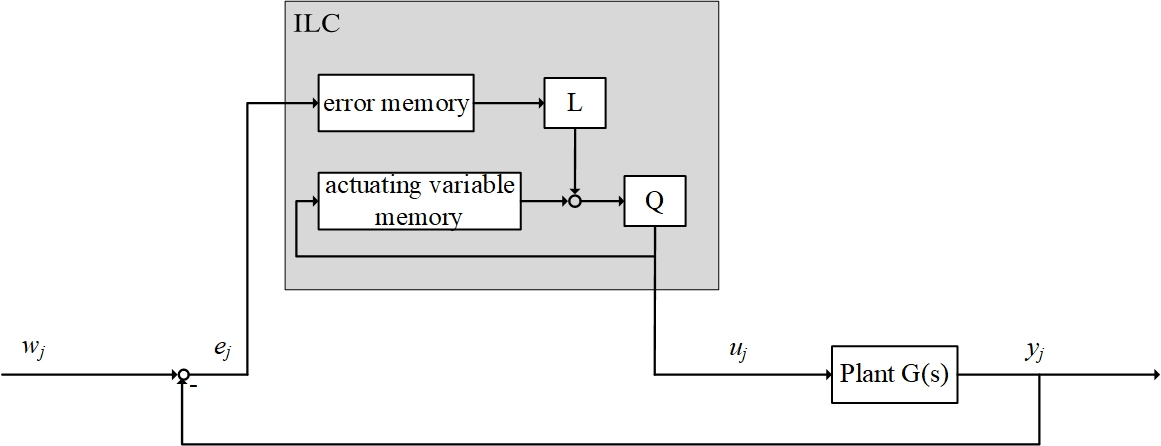
\includegraphics[width=0.9\textwidth]{images/ILC_only.jpg}
   \caption[Standard ILC control loop]{Standard ILC control loop}
   \label{fig:ILC_only}
 \end{figure}
Considering a linear-time-invariant single-input-single-output system, the ILC learning algorithm would be as follows:
\begin{equation}
    u_{j+1}  = Q(q)[u_{j}(k)+L(q)e_{j}(k+1)]
 \label{eq:ILC_standard}
\end{equation}
where $k$ is the time index, $j$ is the iteration index, $Q(q)$ is defined as the Q-Filter and $L(q)$ represents the learning function. The performance error signal $e_{j}$ is defined as
\begin{equation}
    e_{j}  = w_{j}-y_{j}.
 \label{eq:perf_error}
\end{equation}

 Feedback controllers, such as PI-controllers, are only able to include the current changes in control error. By taking into account the information from previous iterations low tracking errors are achievable through an ILC. This results in very high performance, with convergence during the first few iterations. This can be achieved even for systems prone to repeating disturbances and model uncertainties. While feedback control has a lag in transient tracking, due to reacting to inputs and disturbances, ILC, as a feedforward controller, does not. Another advantage of ILC use is that there is no need for disturbances to be known or measured, as long as these signals show repeating behavior during each iteration. Furthermore, through storing signal information during each iteration ILC enables advanced filtering and signal processing of the control error. However, ILC utilization holds some issues in regards to non-repeating disturbances or noise influences. In these cases it may be useful to combine ILC approaches with a feeback controller. A combination of the systems is also recommended if the plant's behavior is not stable. \cite{ILC2} A parallel architecture of a feedback controller in combination with an ILC is illustrated in \figurename~\ref{fig:ILC_parallel}.
 \begin{figure}[h]
    \centering
    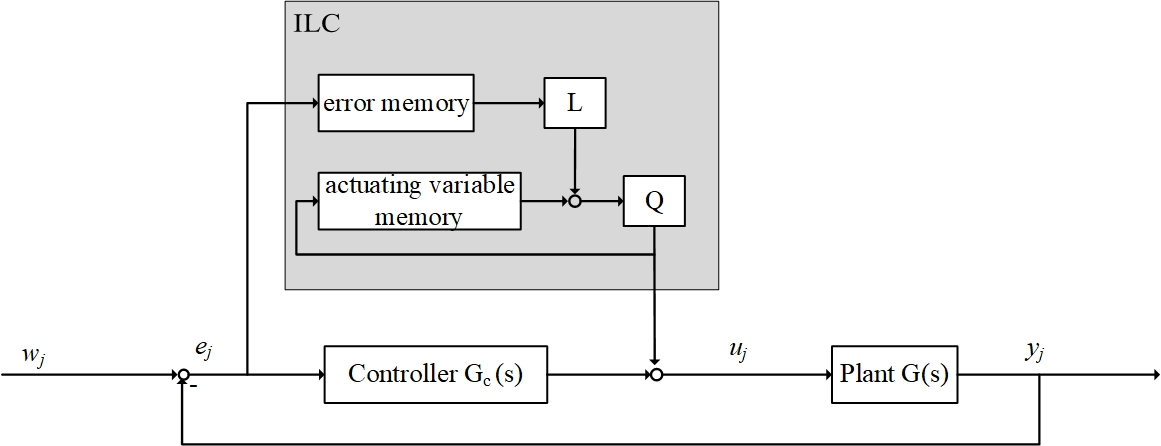
\includegraphics[width=0.9\textwidth]{images/ILC_parallel.jpg}
    \caption[Parallel architecture of ILC with feedback controller]{Parallel architecture of ILC with feedback controller}
    \label{fig:ILC_parallel}
  \end{figure}
\\There are different approaches to designing an ILC. In general, an ILC ideally only learns the repeating disturbance patterns without being influenced by noise. The most common types of ILC learning functions are the P-, D- and PD-type learning functions. As an ILC does have an natural integrator action from one iteration to the next, I-type learning functions are not used that frequently.
\\The discrete-time learning function for a standard PD-type ILC is given as either
\begin{equation}
    u_{j+1}(k) = u_{j}(k)+k_{p}e_{j}(k+1)+k_{d}[e_{j}(k+1)-e_{j}(k)]
 \label{eq:PD_type}
 \end{equation}
 or
 \begin{equation}
     u_{j+1}(k) = u_{j}(k)+k_{p}e_{j}(k)+k_{d}[e_{j}(k+1)-e_{j}(k)].
  \label{eq:PD_type_2}
  \end{equation}
$k_{p}$ represents the proportional gain, while $k_{d}$ is the derivative gain. In case a P-type learning function is implemented the derivation gain is set to $k_{d}=0$. For a D-type learning function $k_{p}=0$ is used, respectively.
\\The performance of these ILC types depends mainly on accurate parameter tuning and does not require an acurate mathematical model of the plant. Despite these approaches being frequently used, there are no tuning guidelines similar to the once mentioned for PI-controller tuning. However, a commonly used way to influence the process behavior is to modify the learning algorithm to include a Q-Filter. This filter can be used to disable learning at high frequiencies, in order to filter high-frequency noise. It furthermore increases robustness. First a filter type, such as Butterworth or Chebyshev, is specified. The bandwith can then be interpreted as a tuning parameter, in addition to the proportional gain $k_{p}$. Initially learning gain and filter bandwidth are set to low values. When a steady baseline behavior and error performance is achieved, the parameter values can be increased to improve performance. The learning gain influences the rate of error convergence, while the Q-Filter influences the error performance. The higher the filter bandwidth, the more increased is the performance. However, this includes a trade-off in robustness. For lower filter bandwidth high robustness can be achieved in a trade-off in performance.
\\Besides the P-,D- and PD-type ILC there are other design approaches. The $H_{\infty}$ method can be used to design a robustly convergent ILC controller, with a trade-off in performance. A quickly converging ILC approach can be achieved by using the plant inversion method. This however depends greatly on an accurate modeling of the plant. The quadratically optimal ILC approach uses quadratic performance criteria to design an optimal ILC. Further information on these alternative design methods is provided in \cite{ILC2}.

\chapter{Modeling and Identification}
\section{Sputnik VAD}
% graphic of Sputnik construction
The Sputnik VAD is an axial-flow blood pump, developed in a cooperative project of the National Research University of Electronic Technology, OJSC Zelenograd Innovation-Technology Center of Medical Equipment, FSBI "Academician V.I. Shumakov Federal Research Center of Transplantology and Artificial Organs", Ministry of Health of Russian Federation, DONA-M LLC and BIOSOFT-M LLC in 2009. \cite{Sputnik1}
\\This device is used for left ventricular assistance in patients with acute heart failure. The therapeutic objective in implantation of a Sputnik VAD is bridging to transplantation. The VAD is able to pump up to 10 liters of blood per minute with a continuous flow profile. The implantable pump weighs about 200 g, has a length of 81 mm and a maximum diameter of 34 mm. It consists of a moving and a stationary part. The moving part, the impeller, which is a rotor with four blades, contains a permanent NdFeB-magnet which is actuated by a brushless DC motor. The rotor spins clockwise with speed values between 4000-10000 rpm. An overview of the pumps specification is presentet in Table \ref{tab:sput1}
\begin{table}[h]
  \centering
  \begin{tabular}{c|c}
    \toprule
    Blood flow  & 0-10 L/min \\
    Rotational speed & 4000-10000 rpm \\
    Length & 81 mm \\
    Diameter & 34 mm \\
    Weight & 200g \\
    \bottomrule
\end{tabular}
  \caption{Specifications of Sputnik VAD}
  \label{tab:sput1}
\end{table}
The stator is located inside a titanium housing with a 16 mm diameter. The stationary part of the pump consists of a flow straightener with three stationary blades and a flow diffusor with three twisted blades. The flow straightener is located in front of the rotor and straightens the incoming blood flow into the rotor. Behind the rotor, the blood is directed into the diffusor. %\cite{Sputnik1}
Figure \ref{fig:sput_cross} depicts a cross-section of the Sputnik VAD and identifies it's individual components.
The connection between the pump and the cardiovascular system is performed using in- and outflow cannulas, a felt ferule and vascular prosthesis which is sewed to the aorta. \cite{Sputnik1}
\begin{figure}[h]
  \centering
  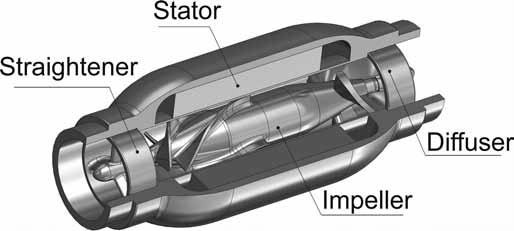
\includegraphics[width=0.6\textwidth]{images/sputnik_cross.png}
  \caption{Cross-section of the Sputnik VAD from \cite{Sputnik6}}
  \label{fig:sput_cross}
\end{figure}
The Sputnik VAD is powered using two lithium-ion batteries, fully loaded providing enough energy for up to eight hours of system support. The maximum charging time for the batteries is less than five hours. During this time the batteries can either be exchanged by another set of batteries or the system can be powered through connection to an AC network. A microprocessor-based driving unit is used to regulate the pump speed, manage the power supply and store parameter data. It is connected percutaneously to the pump with a up to 170 cm long and 5 cm wide lead. \cite{Sputnik1}

\section{Hardware in the Loop Test Bench}
%Aufbau
%Umbau

\section{System Identification}
%Vergleich Flüssigkeiten
%Vergleich Schlauchlängen
%Kennfeld

\chapter{Flow Control}
\section{Controller Design}
\subsection{PI Controller}
\subsubsection{Chien Hrones Reswick}
% Dynamische Messung nutzen
% Werte an Sprungstellen
% Nach Wendetangenten verfahren -> GRAFIK
%Berechnung erklären
\subsection{Iterative Learning Control}
\subsection{Iterative Learning Control with varying iteration length}

\section{Evaluation}
\subsection{PI Controller}
\subsubsection{Chien Hrones Reswick}
% Dynamische Messung nutzen
% Werte an Sprungstellen
% Nach Wendetangenten verfahren -> GRAFIK
%Berechnung erklären
\subsection{Iterative Learning Control}
\subsection{Iterative Learning Control with varying iteration length}
% Kontanten Fluss über verschiedene Druckbereiche?
%
% %Druckverlauf ohne Störung
%
% Herzschlag dazu - Druckverlauf

\chapter{Conclusion and future work}
\section{Conclusion}
As the gap between the incidence of cardiovascular disease and the availability of donor organs will continue to grow in the coming years due to demographic change, it is of increasing importance to further develop alternative therapies for CVDs.
For this reason, a flow control system for the Sputnik VAD axial flow pump was developed in the context of this work, which enables it to follow different predefined flow trajectories.
\\This was achieved by a stepwise development and optimization of a control loop, which has a parallel architecture of a PI controller and an ILC.
\\First, the performance of two PI controllers, designed using the Ziegler Nichols and Chien Hrones Reswick methods, was compared. The second one showed a significantly higher performance, which led to its further use within the ILC implementation as a stabilizing feedback controller.
\\After successful optimization of the Q-filter implemented within the ILC, a series of tests were performed to determine the quality of the ILC. Under the idealized assumption of disturbance by a heartbeat with regular heart rate of $60\, bpm$ and adjustment of the length of the flow trajectories to a duration of $1\,s$ per iteration, satisfactory results were obtained with averaged error values ranging from $RMSE_{\mathrm{rect}}=0.22\,l/min$ for a rectangular trajectory to $RMSE_{\mathrm{sine}}=0.09\,l/min$ for a sinusoidal trajectory. When the standard ILC was subjected to a non-repetitive disturbance in the form of heartbeats of variable heart rates, a significant degradation in performance was evident. For this case, the averaged error values were between $RMSE_{\mathrm{rect}}=0.77\,l/min$ for the rectangular signal and for a constant reference flow even $RMSE_{\mathrm{const}}=1.13\, l/min$.
\\In order to keep the performance of the control high even in the presence of variable disturbances, the ILC was extended by further data preprocessing in the form of resampling the data of the actuating variable of the ILC to an iteration length corresponding to the current heart rate. This allowed the averaged error values for a constant flow to be reduced to just $RMSE_{\mathrm{resampled,const}}=0.05\, l/min$. A noticeable improvement in performance was also achieved for a sinusoidal and a triangular signal. Only for the rectangular signal no clear increase in performance could be seen.
For all four reference trajectories tested, however, the pump stopped after some time because the actuating variable exhibited oscillating behavior.

\section{Future work}
In order to ensure long-term flow control under the influence of non-repeating disturbances, as would be necessary for use on patients, the robustness of the controller to this type of disturbance would have to be optimized.

Conceivable approaches to achieve this goal could be given in the use of other ILC implementation, such as a current iteration learning control as presented in \cite{ILC2}. Also the use of a higher-order learning algorithm, which uses not only the last but also further back iterations for the calculation of the current one, would be recommendable.

One possible hardware improvement with respect to the robustness of the control system would be to use the control unit associated with the Sputnik VAD instead of the ESCON 50/4 EC-S.

For the use of the resampling functionality as implemented in this work to improve the ILC for non-repetitive disorders, the additional analysis of ECG data would be necessary in clinical use.
\\However, since the Sputnik pump is a therapeutic option with the therapeutic goal of bridging to transplantation, it is conceivable that a patient may require prolonged support from the system. In such a case, it would be desirable not to restrict the patient's mobility and quality of life with an additional medical device. For this reason, a further development of the ILC approach, which would make the use of an ECG signal obsolete, would be desirable.



%**********
%* Anhang *√
%**********

\cleardoublepage
\appendix
\chapter{Appendix}
\section{System Identification}\label{A1}
\begin{figure}[ht]
  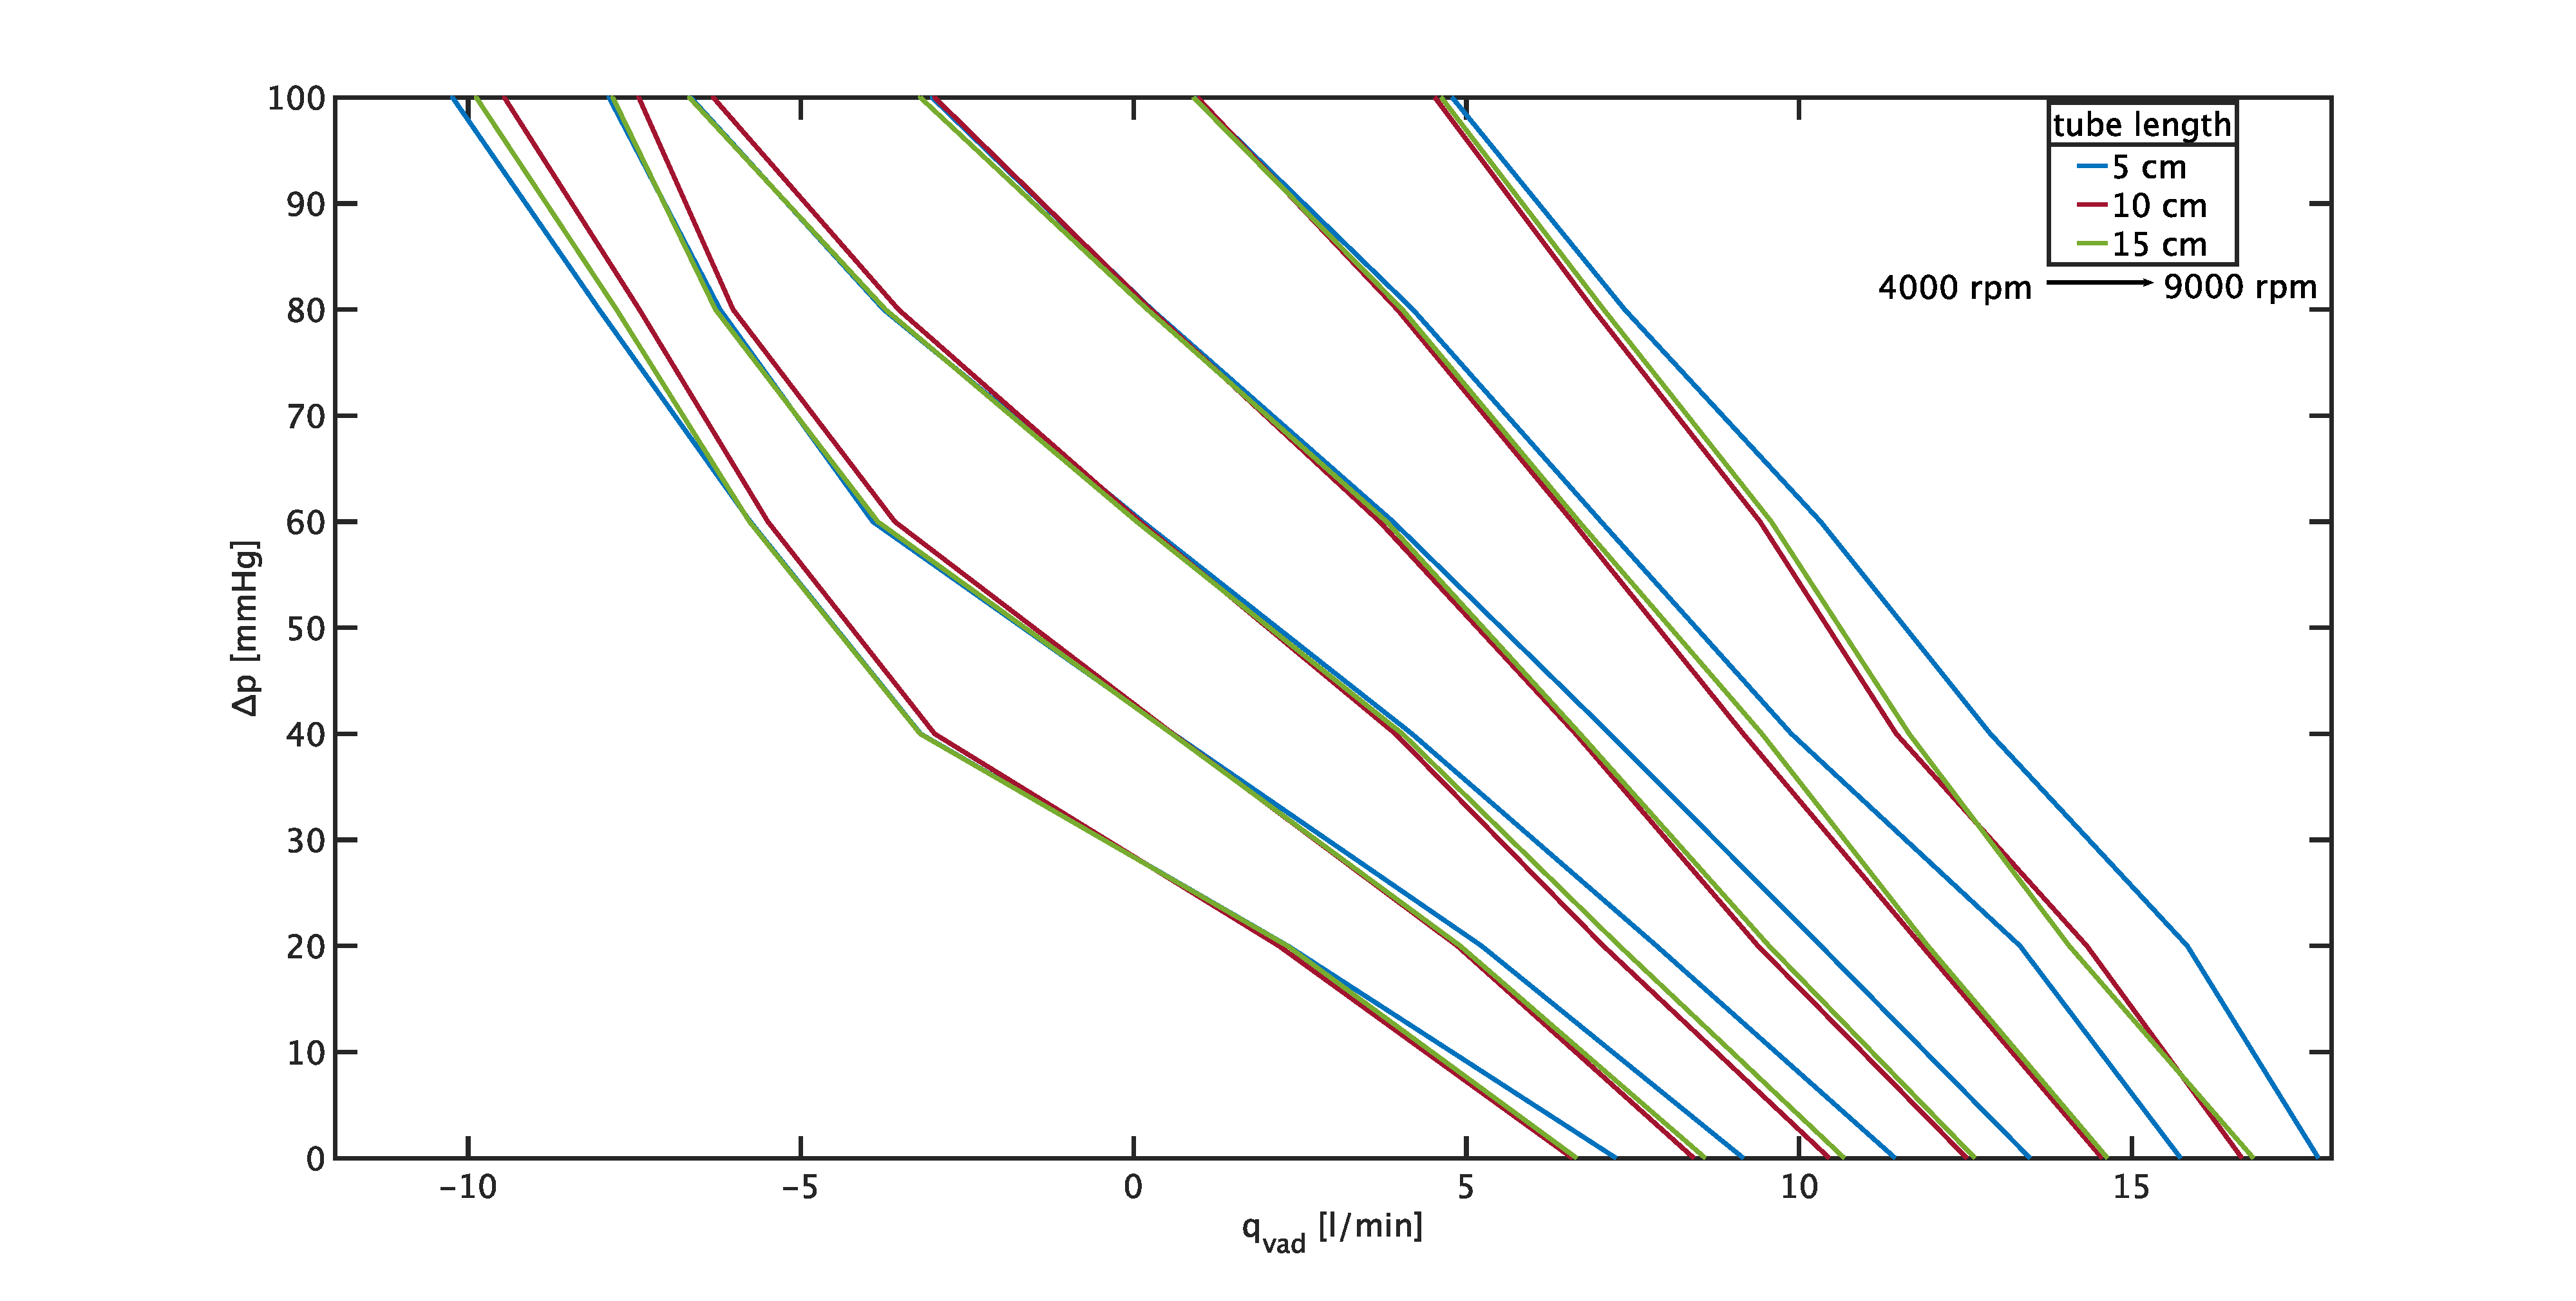
\includegraphics[width=0.9\textwidth]{images/plots_syst_ident/100w_tube_length_new.pdf}
  \caption[Static map for different tube length in 100 \% water]{Static map for varying tube length in 100 \% water}
  \label{fig:anh_1}
\end{figure}

\begin{figure}[ht]
  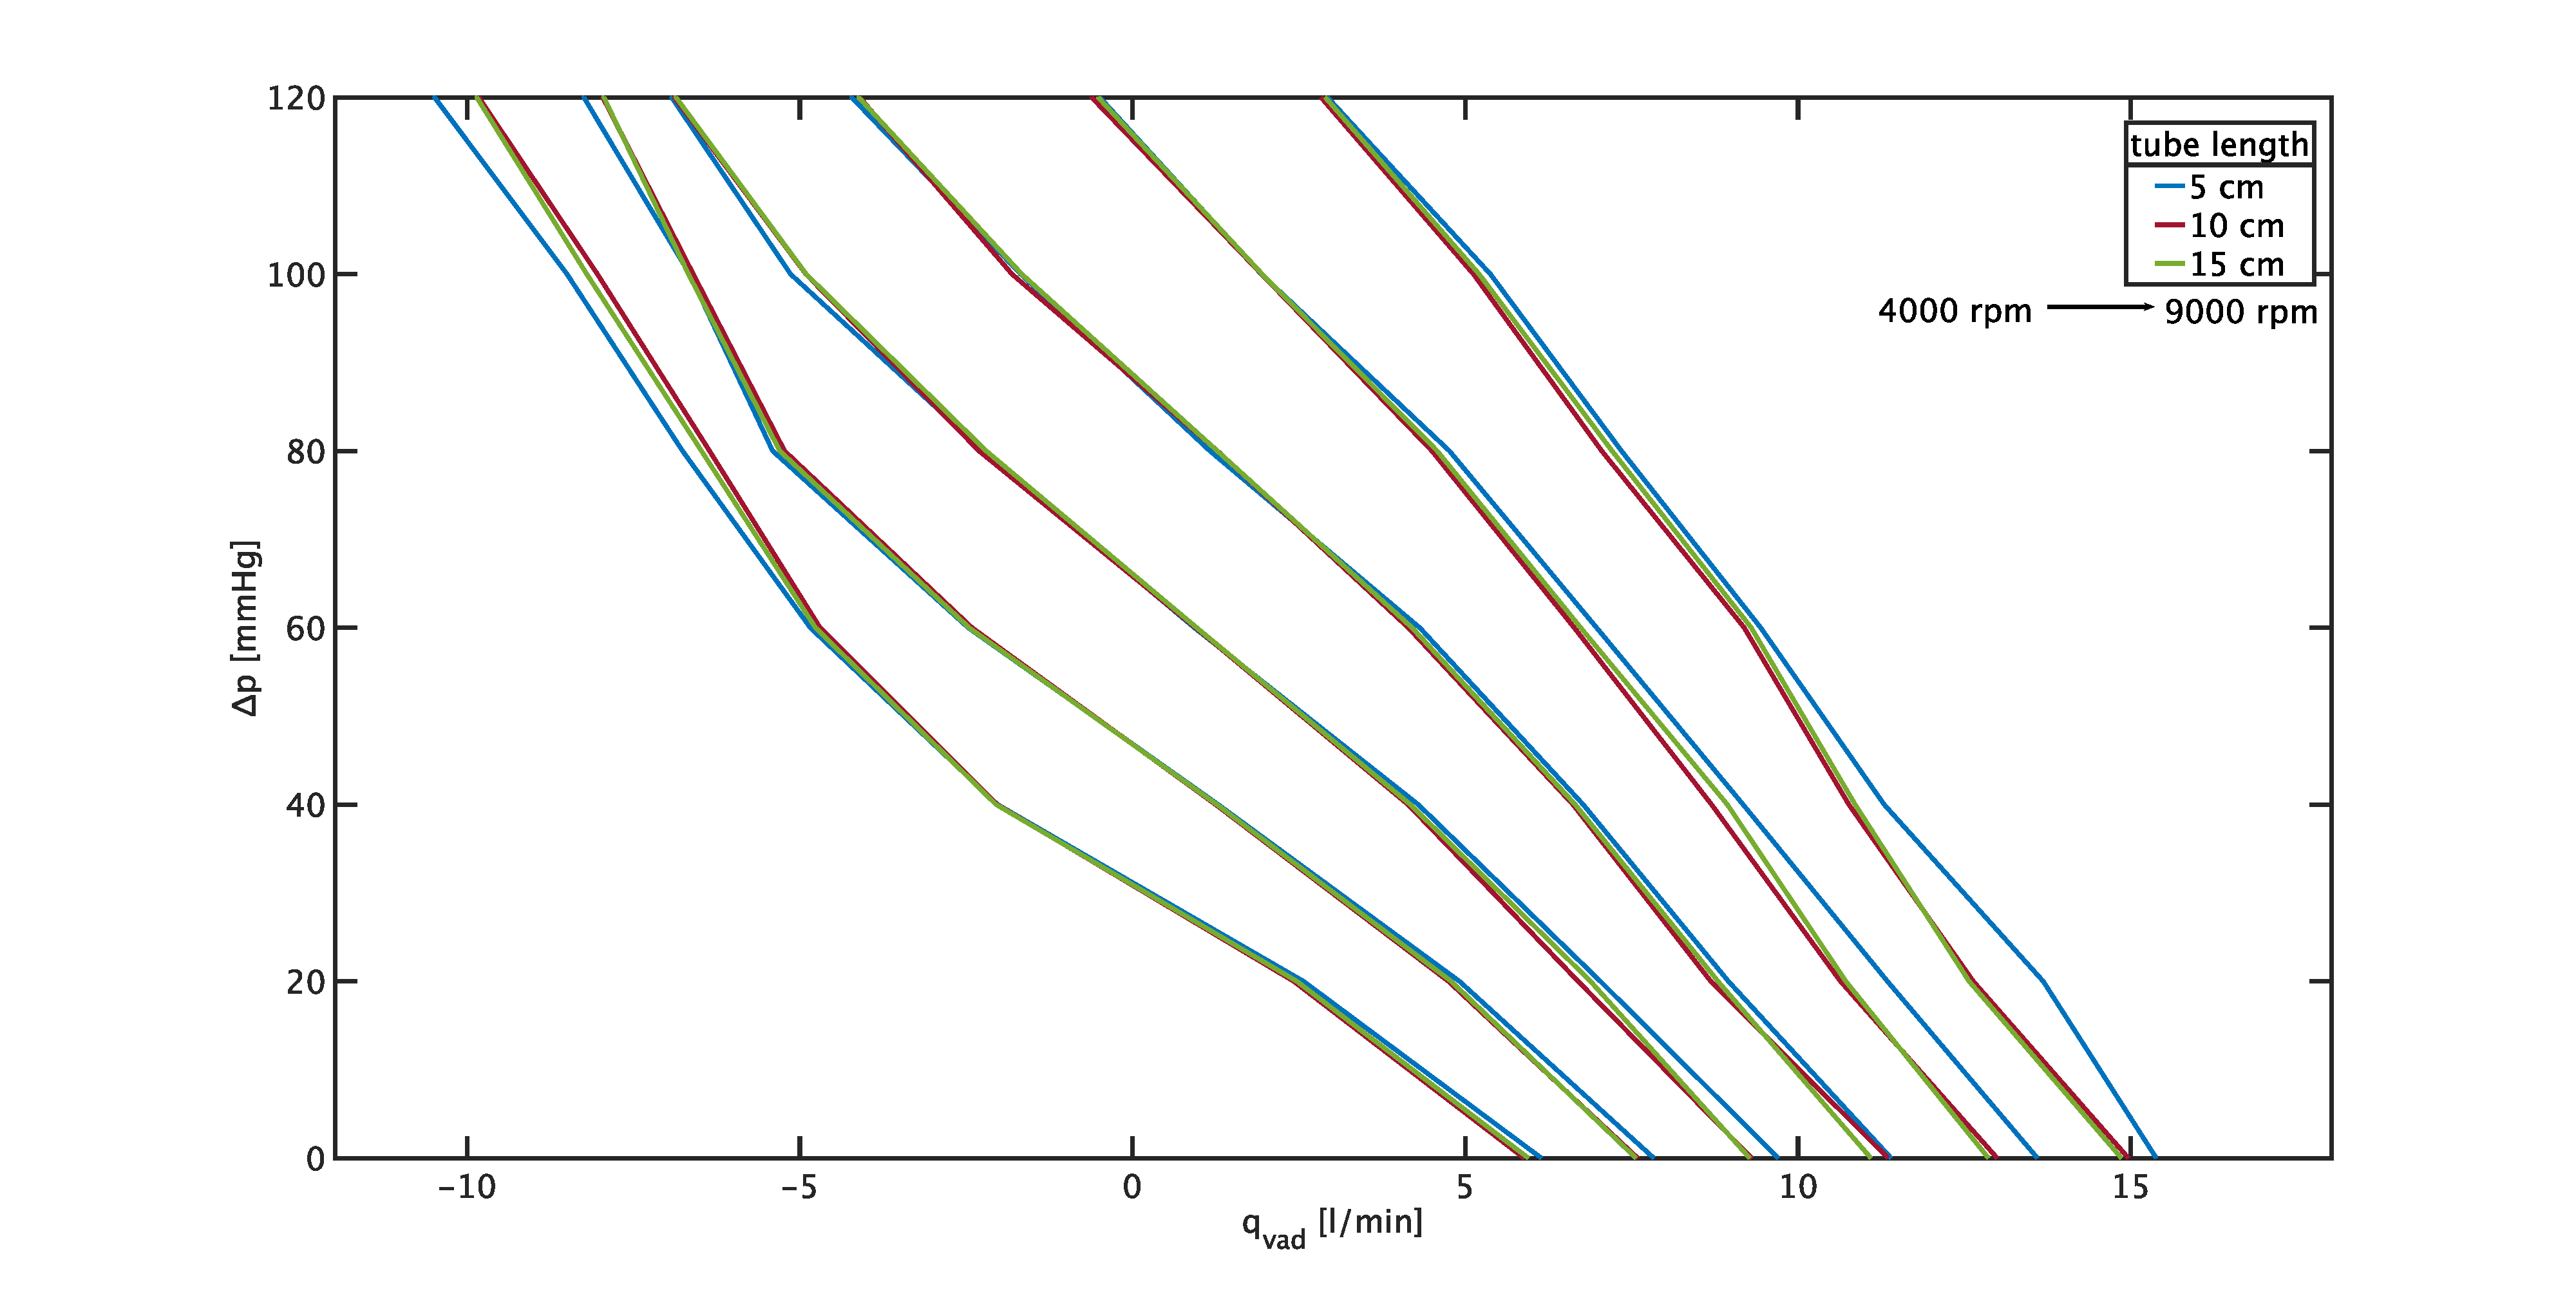
\includegraphics[width=0.9\textwidth]{images/plots_syst_ident/80w20g_tube_length_new.pdf}
  \caption[Static map for different tube length in 80 \% water 20 \% glycerin solution]{Static map for varying tube length in 80 \% water 20 \% glycerin solution}
 \label{fig:anh_2}
\end{figure}

\begin{figure}[ht]
  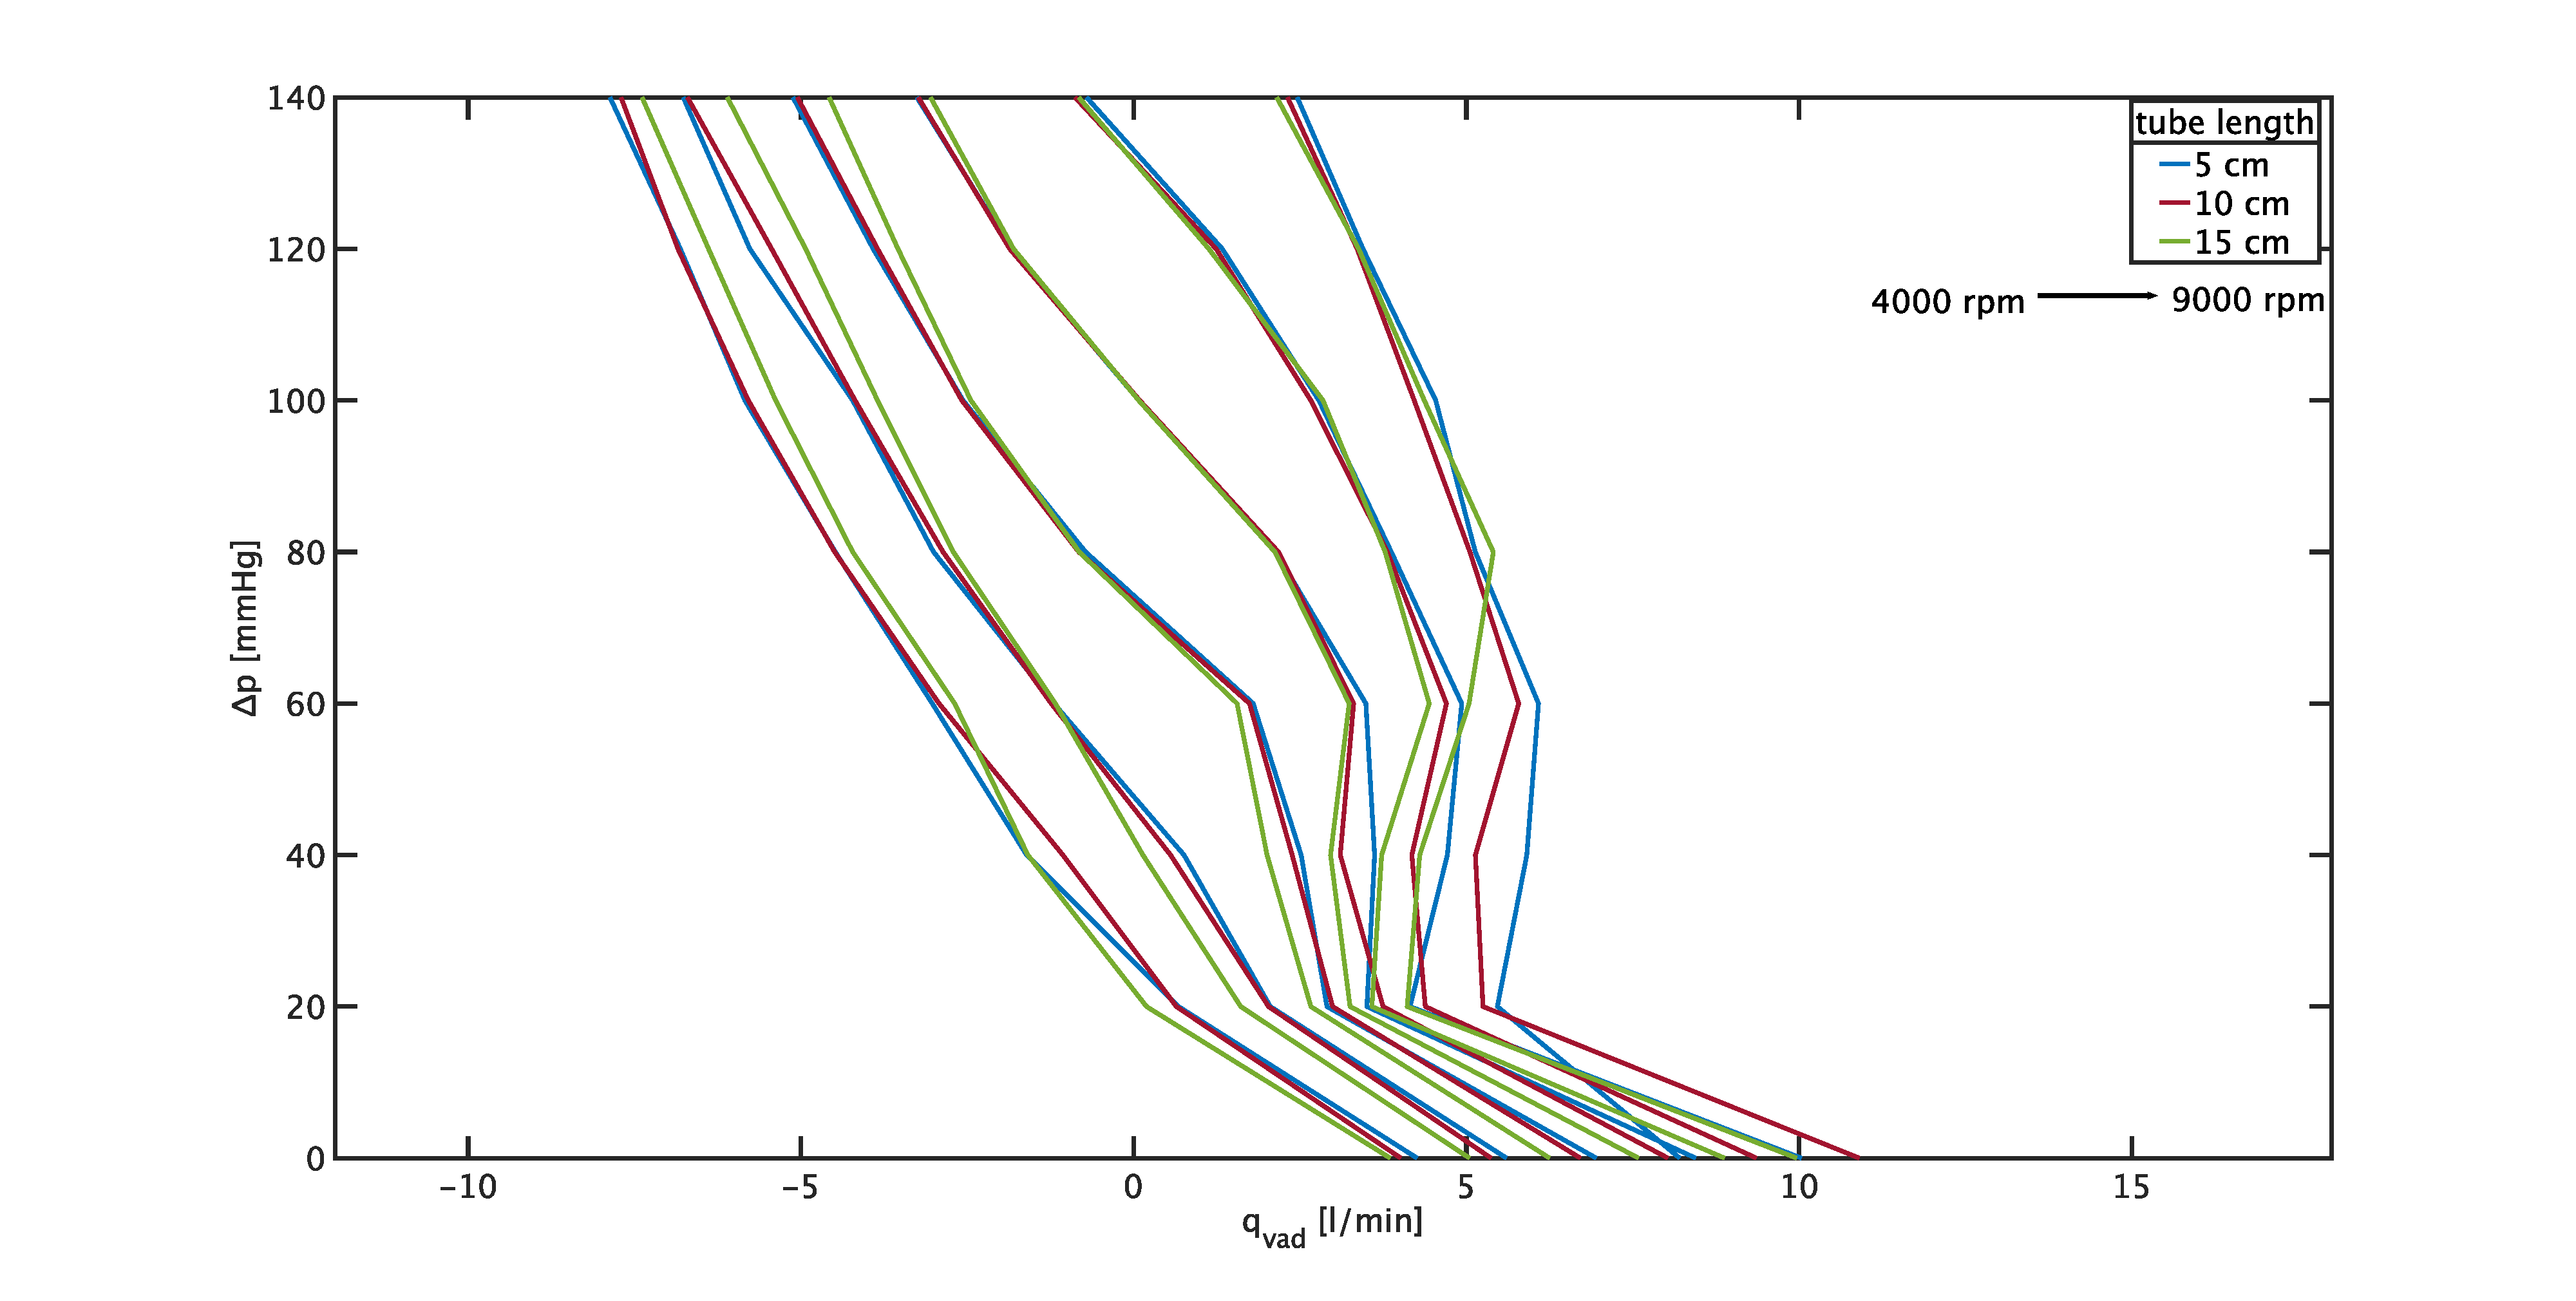
\includegraphics[width=0.9\textwidth]{images/plots_syst_ident/40w60g_tube_length_new.pdf}
  \caption[Static map for different tube length in 40 \% water 60 \% glycerin solution]{Static map for varying tube length in 40 \% water 60 \% glycerin solution}
    \label{fig:anh_3}
\end{figure}

\begin{figure}[ht]
  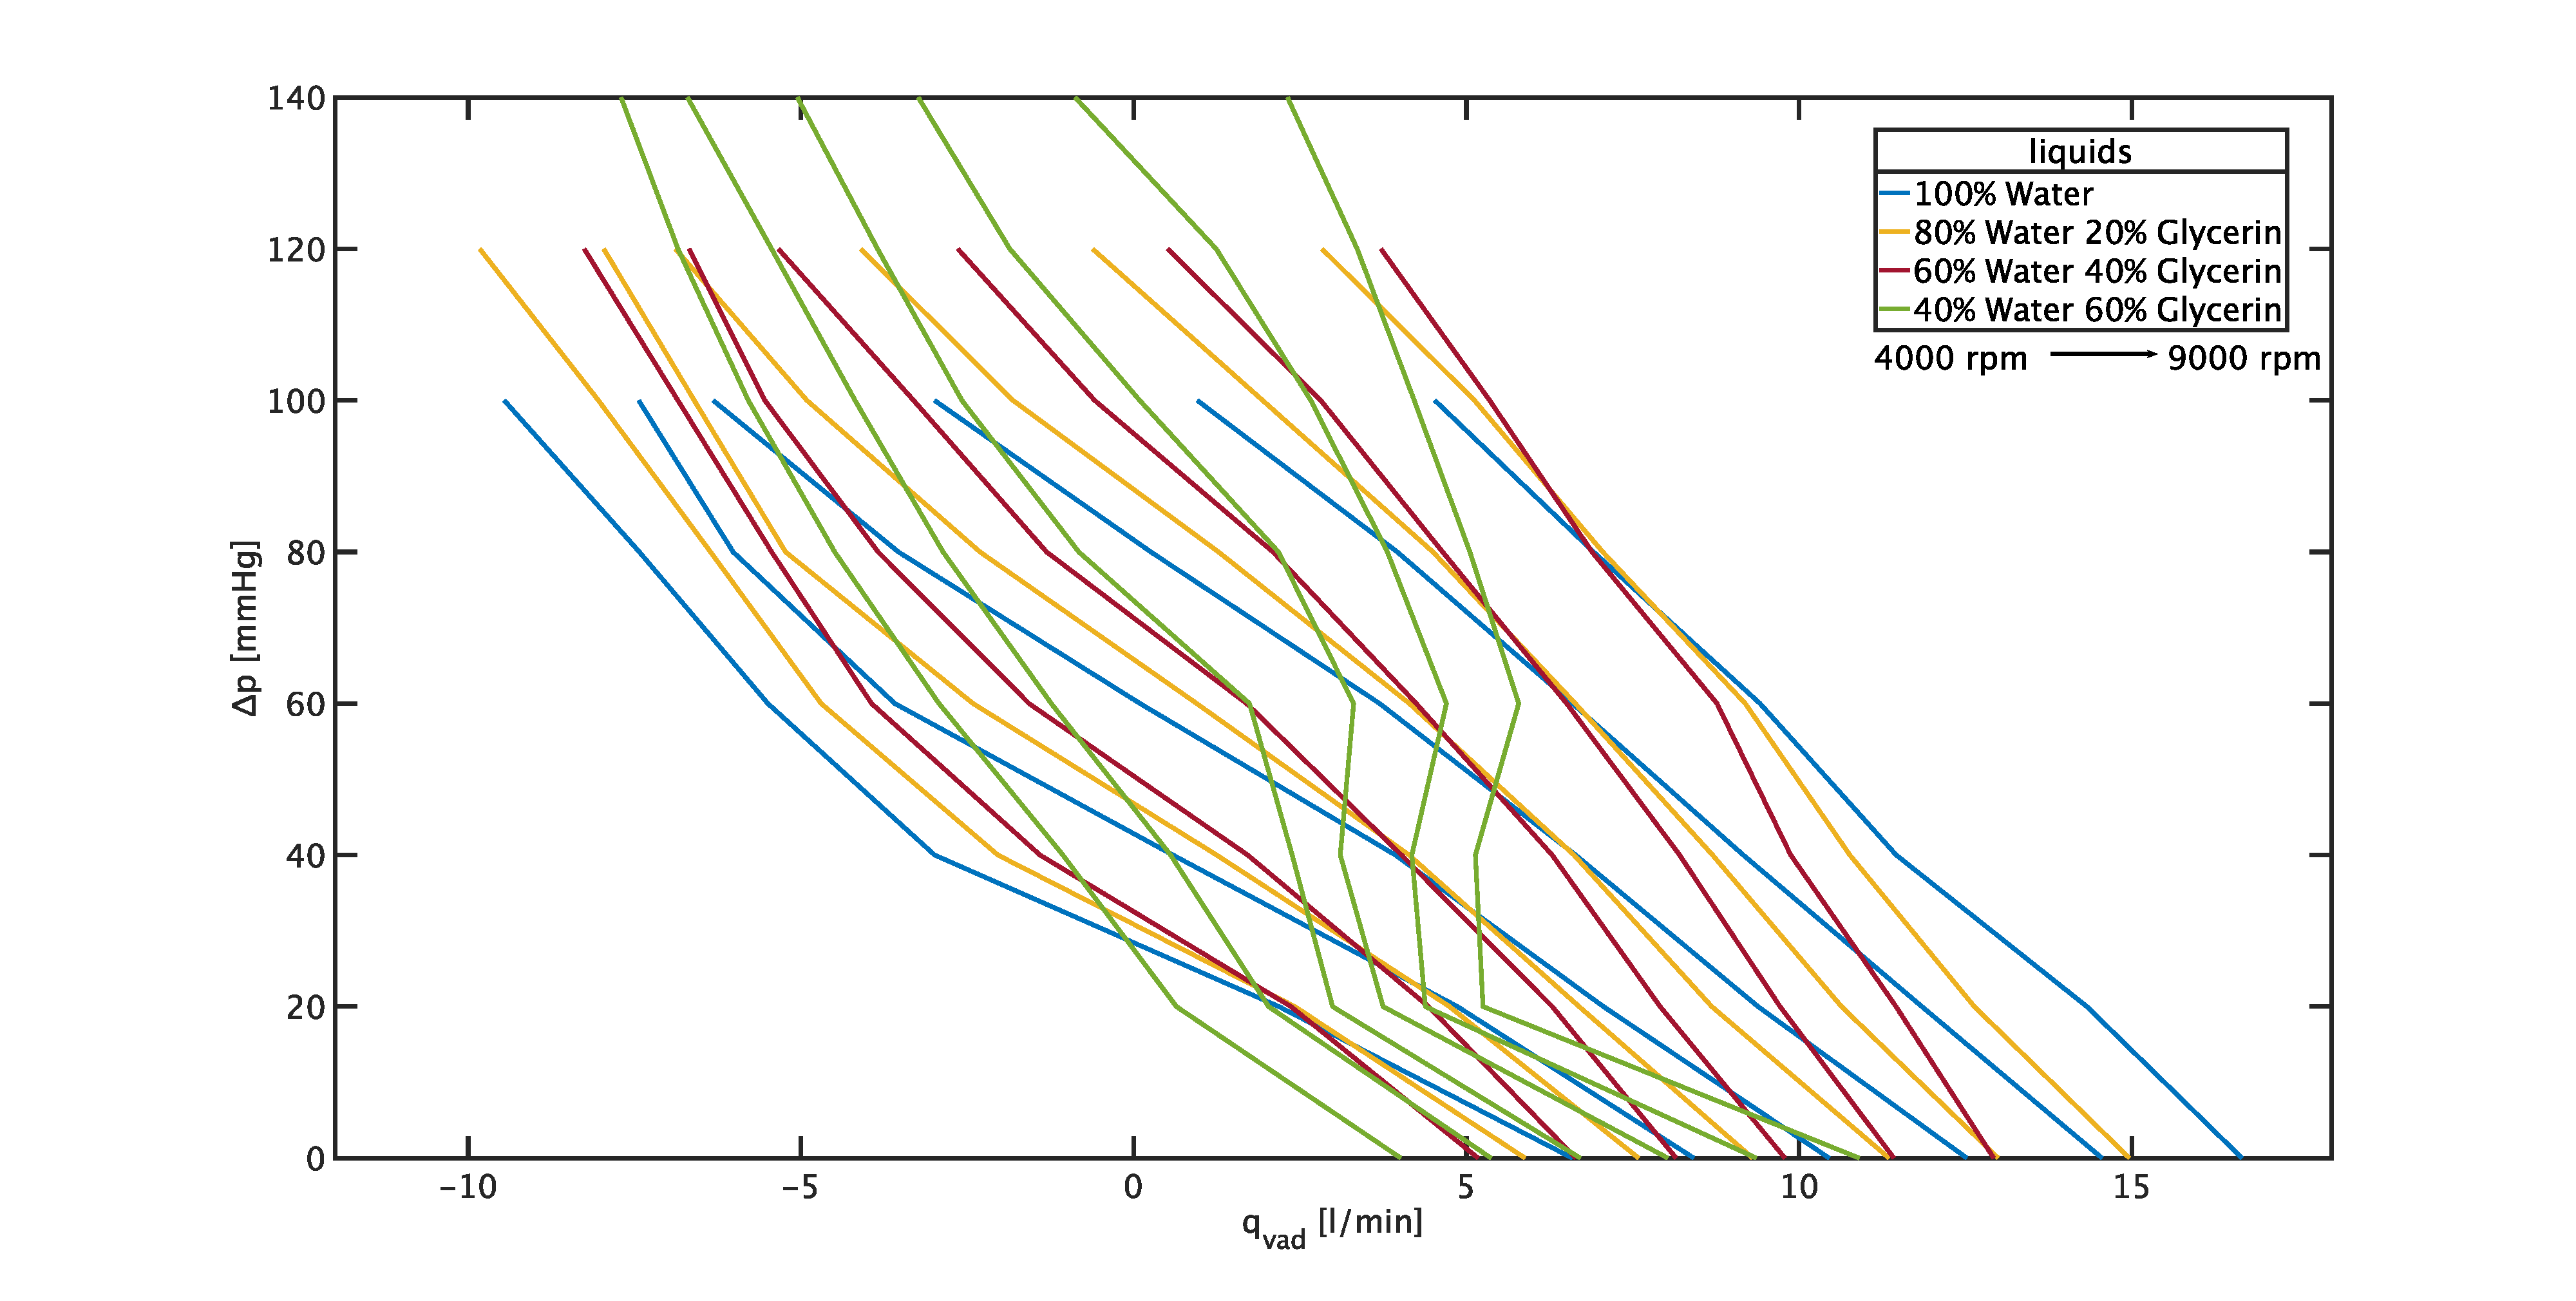
\includegraphics[width=0.9\textwidth]{images/plots_syst_ident/medium_liquid_change_new.pdf}
  \caption[Static map for varying liquid solutions with medium tubes]{Static map for varying liquid solutions with medium tubes}
    \label{fig:anh_4}
\end{figure}

\begin{figure}[ht]
  \includegraphics[width=0.9\textwidth]{images/plots_syst_ident/short_liquid_change_new.pdf}
  \caption[Static map for varying liquid solutions with short tubes]{Static map for varying liquid solutions with short tubes}
    \label{fig:anh_5}
\end{figure}



%**********************************************************
% Literaturverzeichnis (hier muss nichts ge�ndert werden) *
%**********************************************************

\bibliographystyle{alphadin}    %\bibliographystyle{} plain dinat
\bibliography{literatur}%


\end{sloppypar}
\end{document}
